\documentclass[11pt, a4paper, USenglish]{article} % change ``USenglish'' to ``norsk'' if applicable.
\usepackage{tabstackengine}
\stackMath
\usepackage{kyblab} % Contains all included packages. See kyblab.sty.
\usepackage[framed,numbered,autolinebreaks,useliterate]{mcode}
\usepackage{textcomp}
\addbibresource{bibliography.bib} % Makes the bibliography file available to biblatex.
\newcommand{\td}[1]{\dot{\tilde{#1}}}
\newcommand{\tdd}[1]{\ddot{\tilde{#1}}}
\newcommand{\MATLAB}{\textsc{Matlab}\xspace}
\newcommand{\QuaRC}{\textsc{QuaRC}\xspace}
\newcommand{\lin}[2]{\left. \frac{\partial{#1}}{\partial{#2}}\right|_P}
\begin{document}
 

% Titlepage
\title{TTK4115 Helicopter Lab Report}
\author{
    Group 16\\
    Odin Aleksander Severinsen (student number:)\\
    Sigurd Totland (student number: 478437) \\
    Viktor Korsnes (student number:)
}
\date{\today}
\begin{titlepage}
    \maketitle
    \begin{figure}[htb]
        \centering
        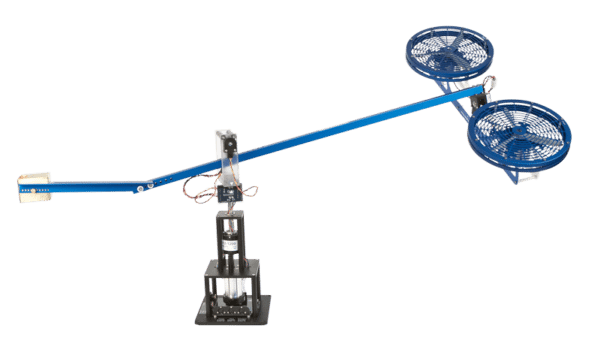
\includegraphics[width=0.65\textwidth]{figures/quanser}
    \end{figure}
    \begin{figure}[b]
        \centering
        
\includegraphics[width=0.5\textwidth]{figures/itk_ntnu}\\
        Department of Engineering Cybernetics
    \end{figure}
    \thispagestyle{empty}
\end{titlepage}

% Abstract
\newpage
\begin{abstract} 
%\addcontentsline{toc}{section}{Abstract} % add this if you want the abstract in the table of contents.
  In this this project a physical helicopter model is controlled using different methods to obtain stability and easy controllability with a joystick. The control methods are all based on a linearized mathematical model of the system. Among them are feed forward control, monovariable feedback control, and feedback control using a linear quadratic regulator (LQR). The latter was done both with direct state feedback and with state estimation using a linear observer. 
\end{abstract}

\thispagestyle{empty} % Avoid page numbering on the abstract page.

% TOC
\newpage
\tableofcontents
\thispagestyle{empty} % Avoid page numbering on the table of contents.

% Main content
\newpage
\setcounter{page}{1}

% Intro

\section{Introduction}\label{sec:intro}
Your introduction should contain an overview of the work you were assigned, as well as a few sentences putting the work into a larger perspective. You should also give a quick description of how the report is organized (as is done below).

You should of course put most of the work into doing good work in the lab and then presenting it in the report. When presenting your work in the report, both content and presentation/layout matters. Since your only way of communicating your good effort in the lab is through writing about it here, the way you write about it is essential. This means that even if you have the very best controller but describe it poorly, you will probably not be rewarded for the good results. A plot showing perfect control is worth very little if it is not accompanied by a clear description of what it represents.

Layout is naturally less important than content, but it still matters. You can think of report writing like selling an apartment; when you present your apartment for potential buyers you will of course clean the apartment and make it good looking. How clean the apartment is does of course not determine its value, but it is still important since it influences the subjective value your buyers will put on the apartment. 

\subsection{Software}
You are of course free to use whatever software you want for report writing. You can also submit a handwritten report, although this is probably not a great idea if your handwriting can be hard to read. 

You can also use Word or a similar word processor. However, it is next to impossible to achieve decent layout with Word. The support for vector graphics (discussed later) is extremely poor, and text tends to look pretty bad (bad support for kerning and ligatures). Furthermore, math is both time consuming and difficult to input, and tends to look very ugly. In general, a report written in Word looks like a draft.

It is strongly recommended to use Latex. Unless you tweak the layout too much, your report will almost certainly look very good. Although it can take a bit of effort to get started, it is also much quicker to use than Word and similar programs. The support for math and vector graphics is also great.

If you are new to Latex, you can have a look at the source for this document to get started. You can also look at the presentation by~\cite{Berland2010} (in Norwegian) or consult~\cite{Oetiker2011}. Another good reason to learn Latex is that you probably don't want to write your master's thesis in something like Word, doing so would likely be very frustrating. Being reasonably fluent in Latex before you get that far will make your thesis work much smoother.

Some of you are probably fluent in Latex and might plan to write the report using it. Please resist the temptation (if any) to change the fonts, make super fancy headers (they are not necessary for a report like this), change the margins, change the paragraph indentation and/or spacing, and similar things.

A great tool for collaborating on Latex documents is ShareLaTeX at \url{https://www.sharelatex.com/}; if you use this you won't have to install anything on your computer. Texmaker at \url{http://www.xm1math.net/texmaker/} is a good cross-platform editor. Some people like Lyx, which is a Latex editor that behaves a little bit like Word. If you prefer to compile your Latex document on the command line, the latexmk \url{https://www.ctan.org/pkg/latexmk} command is a great tool included in most TeX distributions. There is also a simple Vim plugin that uses latexmk as its backend called LaTeX-BoX \url{https://github.com/LaTeX-Box-Team/LaTeX-Box}.

\subsection{Other Comments}
Unless you have a very good reason not to, you should write the report in English. If you have problems with Latex, the solution is usually just a few Google searches away.

This report is organized as follows: \Cref{sec:prob_descr} contains some course specific equations, and some tips on how to create illustrations. Several \LaTeX{} tips can be found in \Cref{sec:latex_tips}, such as how to create a table and matrix equations. \Cref{sec:figures} contains some advice on using plots from MATLAB\@. The closing remarks are in~\Cref{sec:conclusion}, respectively. \Cref{sec:matlab} contains a MATLAB file while \Cref{sec:simulink} shows an example Simulink diagram. The Bibliography can be found at the end, on page~\pageref{sec:bibliography}.


%%%%%%%%%%%%%%%%%%%%%%%%%%%%%%%%%%%%%%%%%%%%%%%%%%%%%%%%%%%%%%%%%%%%

%  Part I
\section{Problems}\label{sec:figures}
\subsection{Part I - Mathematical modelling}\label{subsec:part1}
\subsubsection{Problem 1}

In the following derivations, Newton's $2^{\text{nd}}$ law of motion for rotation is used:

\begin{equation}\label{eq:P1_N2}
    J \dot{\omega} = \sum \tau = \sum \left(r\cdot F\right)
\end{equation}
Additionally, the definitions
\begin{subequations}\label{eq:P1_Vd_Vs_definitions}
    \begin{align}
        V_d &= V_f - V_b\label{eq:P1_Vd_definition} \\
        V_s &= V_f + V_b\label{eq:P1_Vs_definition}
    \end{align}    
\end{subequations}
are introduced to simplify the derived equations. Lastly, it is assumed that the moments of inertia about the pitch, elevation and travel axis is, respectively

\begin{subequations}\label{eq:P1_moments_of_inertia}
    \begin{align}
        J_p &= 2m_pl_p^2 \label{eq:P1_moment_of_inertia_p} \\
        J_e &= m_cl_c^2 + 2m_pl_h^2 \label{eq:P1_moment_of_inertia_e} \\
        J_{\lambda} &= m_cl_c^2 + 2m_p(l_h^2 + l_p^2) \label{eq:P1_moment_of_inertia_lambda}
    \end{align}
\end{subequations}
and where all constants used are according to~\cref{fig:heli_dimensions}.

The equations of motion about the pitch axis can be computed by using~\cref{eq:P1_N2},~\cref{fig:heli} and \cref{eq:P1_forces_propellers}. The forces that generate a moment about the pitch axis are the forces generated by the motors, $F_f = K_f V_f$ and $F_b = -K_f V_b$, and their weight decomposed, $F_{g,f}=-m_pg\cos(p)$ and $F_{g,b}=m_pg\cos(p)$ according to~\cref{eq:P1_weight_m_p}, where the forces are signed according to~\cref{fig:heli}. Given the discussed considerations, the equation of motion for rotation about the pitch axis can be derived as follows:

\begin{align}\label{eq:P1_pitch_non-linear}
    J_p \ddot{p} &= l_p F_f - l_p F_b \nonumber \\
    J_p \ddot{p} &= l_p K_f V_f - l_p K_f V_b \nonumber \\
    J_p \ddot{p} &= l_p K_f (V_f - V_b) \nonumber \\
    J_p \ddot{p} &= L_1 V_d
\end{align}
where the definition
\begin{equation}\label{eq:P1_L_1}
    L_1 = l_p K_f
\end{equation}
is introduced.

For the elevation, the same procedure as for pitch is used by considering how the motor forces' components about the elevation axis are a function of $p$ and that the weight of the motors and the counterweight have arms that are functions of $e$. This yields:

\begin{align}\label{eq:P1_elevation_non-linear}
    J_e \ddot{e} &= g l_c m_c \cos{e} - 2 g l_h m_p \cos{e} + K_f l_h V_f \cos{p} + K_f l_h V_b \cos{p} \nonumber \\
    J_e \ddot{e} &= L_2 \cos{e} + L_3 V_s \cos{p}
\end{align}
where the definitions
\begin{equation}\label{eq:P1_L_2}
    L_2 = g (l_c m_c - 2 l_h m_p)
\end{equation}
and
\begin{equation}
    L_3 = K_f l_h
\end{equation}
are made.

Finally, to calculate travel, one needs to consider only the motor forces as they are the only considered forces able to generate moment about the travel axis. This component is a function of $p$. Additionally, the arm is a function of $e$. In total, this yields:

\begin{align}\label{eq:P1_travel_non-linear}
    J_\lambda \ddot{\lambda} &= -(K_f l_h V_f + K_f l_h V_b)\cos{e}\sin{p} \nonumber \\
    J_\lambda \ddot{\lambda} &= L_4 V_s \cos{e} \sin{p}
\end{align}
Here, the definition
\begin{equation}\label{eq:P1_L_4}
    L_4 = - K_f l_h
\end{equation}
is made.

The reason for the negative sign is because a positive pitch gives a negative travel rate, in accordance to~\cref{fig:heli}. 
Summarised
\begin{subequations}\label{eq:P1_equation_of_motion}
    \begin{align}
        \ddot{p} &= \frac{L_1 V_d}{J_p} 
        \label{eq:P1_p_motion} \\
        \ddot{e} &= \frac{L_2 \cos{e} + L_3 V_s \cos{p}}{J_e} 
        \label{eq:P1_e_motion} \\
        \ddot{\lambda} &= \frac{L_4 V_s \cos{e} \sin{p}}{J_\lambda}
        \label{eq:P1_lambda_motion}
    \end{align}
\end{subequations}
\subsubsection{Problem 2}
In this part we wish to linearise at the point $\mathbf{x^*} = [~p^*\quad e^*\quad\lambda^*~]^T =
[~0\quad0\quad0~]^T$ and $\mathbf{u^*} = [~V_s^*\quad V_d^*~]^T$ where
\begin{equation*}
    \begin{bmatrix}
        \tilde{p} \\
        \tilde{e} \\
        \tilde{\lambda} \\
    \end{bmatrix}
    =
    \begin{bmatrix}
        p \\
        e \\
        \lambda \\
    \end{bmatrix}
    -
    \begin{bmatrix}
        p^* \\
        e^* \\
        \lambda^* \\
    \end{bmatrix}
\quad\text{and}\quad
    \begin{bmatrix}
        \tilde{V_s} \\
        \tilde{V_d} 
    \end{bmatrix}
    =
    \begin{bmatrix}
        V_s \\
        V_d
    \end{bmatrix}
    -
    \begin{bmatrix}
        V_s^* \\
        V_d^*
    \end{bmatrix}
\end{equation*}
is a coordinate transformation introduced to simplify further analysis. The linearisation will be with the helicopter horizontal in both pitch and elevation, as well as no travel (see~\cref{fig:heli} to see how angles are defined). For the equilibrium point, $V_d^*$ and $V_s^*$ needs to be determined. An equilibrium point implies that $\dot{p}=\dot{e}=\dot{\lambda}=0$, which again implies that $\dot{\dot{p}}=\dot{\dot{e}}=\dot{\dot{\lambda}}=0$. Based on this and ~\cref{eq:P1_pitch_non-linear}, one can deduce that $V_d^*$ will be zero, as anything else would eventually give a $\dot{p} \neq 0$ as $t\to\infty$.

To derive $V_s^*$ it is possible to use~\cref{eq:P1_elevation_non-linear}:

\begin{align*}
     J_e \ddot{e} &= L_2 \cos{e} + L_3 V_s \cos{p}\bigg{|}_{\mathbf{x}=\mathbf{x^*}} \\
     \implies\quad J_e\cdot0 &= L_2\cdot1 + L_3V_s^*\cdot1 \\
     V_s^* &= -\frac{L_2}{L_3} \\
     V_s^* &= -\frac{g(l_c m_c - 2 l_h m_p)}{K_f l_h}
\end{align*}
To summarise:
\begin{subequations}
    \begin{align}
        V_s^* &= -\frac{g(l_c m_c - 2 l_h m_p)}{K_f l_h} \label{eq:P1p2_Vs_asterix} \\
        V_d^* &= 0 \label{eq:P1p2_Vd_asterix}
    \end{align}    
\end{subequations}
To simplify further analysis, the following coordinate transformation is introduced.
\begin{equation}
    \begin{bmatrix}
        \tilde{p} \\ \tilde{e} \\ \tilde{\lambda}
    \end{bmatrix}
    =
    \begin{bmatrix}
        p \\ e \\ \lambda
    \end{bmatrix}
    -
    \begin{bmatrix}
        p^* \\ e^* \\ \lambda^*
    \end{bmatrix}
    \quad \text{and} \quad
    \begin{bmatrix}
        \tilde{V}_s \\ \tilde{V}_d
    \end{bmatrix}
    =
    \begin{bmatrix}
        V_s \\ V_d
    \end{bmatrix}
    -
    \begin{bmatrix}
        V_s^* \\ V_d^*
    \end{bmatrix}
\end{equation}
Which gives the following motion equations.
\begin{equation}
    \begin{bmatrix}
        p \\ e \\ \lambda
    \end{bmatrix}
    =
    \begin{bmatrix}
        \tilde{p} \\ \tilde{e} \\ \tilde{\lambda}
    \end{bmatrix}
    \quad \text{and} \quad
    \begin{bmatrix}
        V_s \\ V_d
    \end{bmatrix}
    =
    \begin{bmatrix}
        \tilde{V}_s \\ \tilde{V}_d
    \end{bmatrix}
    +
    \begin{bmatrix}
        -\frac{L_2}{L_3} \\ 0
    \end{bmatrix}
\end{equation}
To linearise, we use the Jacobian and evaluate in our equilibrium
\begin{equation}
    a_{i,j} = \left. \frac{\partial f_i}{\partial x_j} \right 
    |_{\tilde{p} = \tilde{e} = \tilde{\lambda} = 0}
\end{equation}

Where $f_i$ represents the function from problem 1, \cref{eq:P1_equation_of_motion} and $x_j$ represents the states.
We define the following point $P = (\tilde{p} = 0, \tilde{e} = 0, \tilde{\lambda} = 0)$
From this the matrices become
\begin{equation}
    \begin{bmatrix}
        \td{p} \\ \tdd{p} \\ \td{e} \\ \tdd{e} \\
        \td{\lambda} \\ \tdd{\lambda}
    \end{bmatrix}
    =
    \setstackgap{L}{2.1\baselineskip}
    \fixTABwidth{T}
    \bracketMatrixstack{
        \lin{\td{p}}{\tilde{p}} &\lin{\td{p}}{\td{p}} 
        &\lin{\td{p}}{\tilde{e}} &\lin{\td{p}}{\td{e}} 
        &\lin{\td{p}}{\tilde{\lambda}} &\lin{\td{p}}{\td{\lambda}} \\
        \lin{\tdd{p}}{\tilde{p}} &\lin{\tdd{p}}{\td{p}} 
        &\lin{\tdd{p}}{\tilde{e}} &\lin{\tdd{p}}{\td{e}} 
        &\lin{\tdd{p}}{\tilde{\lambda}} &\lin{\tdd{p}}{\td{\lambda}} \\
        \lin{\td{e}}{\tilde{p}} &\lin{\td{e}}{\td{p}} 
        &\lin{\td{e}}{\tilde{e}} &\lin{\td{e}}{\td{e}} 
        &\lin{\td{e}}{\tilde{\lambda}} &\lin{\td{e}}{\td{\lambda}} \\
        \lin{\tdd{e}}{\tilde{p}} &\lin{\tdd{e}}{\td{p}} 
        &\lin{\tdd{e}}{\tilde{e}} &\lin{\tdd{e}}{\td{e}} 
        &\lin{\tdd{e}}{\tilde{\lambda}} &\lin{\tdd{e}}{\td{\lambda}} \\
        \lin{\td{\lambda}}{\tilde{p}} &\lin{\td{\lambda}}{\td{p}}
        &\lin{\td{\lambda}}{\tilde{e}} &\lin{\td{\lambda}}{\td{e}}
        &\lin{\td{\lambda}}{\tilde{\lambda}} &\lin{\td{\lambda}}{\td{\lambda}} \\
        \lin{\tdd{\lambda}}{\tilde{p}} &\lin{\tdd{\lambda}}{\td{p}}
        &\lin{\tdd{\lambda}}{\tilde{e}} &\lin{\tdd{\lambda}}{\td{e}}
        &\lin{\tdd{\lambda}}{\tilde{\lambda}} &\lin{\tdd{\lambda}}{\td{\lambda}}
    }
    \begin{bmatrix}
        \tilde{p} \\ \td{p} \\ \tilde{e} \\ \td{e} \\
        \tilde{\lambda} \\ \td{\lambda}
    \end{bmatrix}
    +
    \setstackgap{L}{2.1\baselineskip}
    \fixTABwidth{T}
    \bracketMatrixstack{
        \lin{\td{p}}{\tilde{V}_s} &\lin{\td{p}}{\tilde{V}_d}  \\
        \lin{\tdd{p}}{\tilde{V}_s} &\lin{\tdd{p}}{\tilde{V}_d}  \\
        \lin{\td{e}}{\tilde{V}_s} &\lin{\td{e}}{\tilde{V}_d}  \\
        \lin{\tdd{e}}{\tilde{V}_s} &\lin{\tdd{e}}{\tilde{V}_d}  \\
        \lin{\td{\lambda}}{\tilde{V}_s} &\lin{\td{\lambda}}{\tilde{V}_d} \\
        \lin{\tdd{\lambda}}{\tilde{V}_s} &\lin{\tdd{\lambda}}{\tilde{V}_d}
    }
    \begin{bmatrix}
        \tilde{V}_s \\ \tilde{V}_d
    \end{bmatrix}
\end{equation}
With values
\begin{equation}
    \begin{bmatrix}
        \td{p} \\ \tdd{p} \\ \td{e} \\ \td{e} \\
        \td{\lambda} \\ \td{\lambda}
    \end{bmatrix}
    =
    \setstackgap{L}{1.05\baselineskip}
    \fixTABwidth{T}
    \bracketMatrixstack{
        0   &1  &0  &0  &0  &0 \\
        0   &0  &0  &0  &0  &0 \\
        0   &0  &0  &1  &0  &0 \\
        0   &0  &0  &0  &0  &0 \\
        0   &0  &0  &0  &0  &1 \\
        -\frac{L_4 L_2}{J_\lambda L_3}  &0   &0   &0   &0   &0 
    }
    \begin{bmatrix}
        \tilde{p} \\ \td{p} \\ \tilde{e} \\ \td{e} \\
        \tilde{\lambda} \\ \td{\lambda}
    \end{bmatrix}
    +
    \setstackgap{L}{1.05\baselineskip}
    \fixTABwidth{T}
    \bracketMatrixstack{
        0                   &0               \\
        \frac{L_1}{J_p}     &0               \\
        0                   &0               \\
        0                   &\frac{L_3}{J_e} \\
        0                   &0               \\
        0                   &0              
    }
    \begin{bmatrix}
        \tilde{V}_s \\ \tilde{V}_d
    \end{bmatrix}
\end{equation}
This simplifies to
\begin{subequations}\label{eq:P1_linearised_equations_of_motion}
    \begin{align}
        \td{p} &= \td{p} \nonumber \\ 
        \tdd{p} &= K_1 \tilde{V}_s \label{eq:P1_linearised_equation_of_motion_p_ddot} \\
        \td{e} &= \td{e} \nonumber \\
        \tdd{e} &= K_2 \tilde{V}_d \label{eq:P1_linearised_equation_of_motion_e_ddot} \\
        \td{\lambda} &= \td{\lambda} \nonumber \\
        \tdd{\lambda} &= K_3 \tilde{p} \label{eq:P1_linearised_equation_of_motion_lambda_ddot}
    \end{align}
\end{subequations}    
Where
\begin{subequations}
    \begin{align}
        K_1 &= \frac{L_1}{J_p} \label{eq:P1_lin_K1} \\
        K_2 &= \frac{L_3}{J_e} \label{eq:P1_lin_K2} \\
        K_3 &= -\frac{L_4 L_2}{J_\lambda L_3} \label{eq:P1_lin_K3}
    \end{align}
\end{subequations}
\subsubsection{Problem 3}
Controlling the helicopter with feed forward is very difficult. 
This stems from an inaccurate model. The model has multiple simplifications compared to the actual system.

\subsubsection{Problem 4}
In order to implement the controllers required in the later parts, the encoder outputs from the helicopter need to be converted from degrees to radians. This is done by adding gains of value $\frac{\pi}{180\degree}$ to the outputs. These gains, labeled D2R can be seen in most of the simulink diagrams in \Cref{sec:simulink}, for example in \cref{fig:P2p2_simulink}.

Furthermore, since the elevation is defined to be zero when the helicopter is horizontal, an offset voltage $V_s^*$ is needed. This voltage was measured by slowly increasing the voltage $V_s$ with the joystick, all the while restraining the other two axes to zero by holding the helicopter loosely at its head. By doing so in a controlled manner, the voltage offset was found to be 
\begin{equation}
    \label{eq:P1_Vs_asterix_value}
    V_s^* \approx 6.5 \volt.
\end{equation}

From the voltage offset, the motor force constant $K_f$ can be calculated. By rearranging \cref{eq:P1p2_Vs_asterix} and inserting values for the constants, $K_f$ can be calculated to be
\begin{equation}
    K_f = -\frac{g(l_c m_c - 2 l_h m_p)}{V_s^* l_h} \approx 0.1537 \frac{\newton \meter}{\sqrt{\watt}}.
\end{equation}
The constant values can be found in \cref{tab:parameters} in \Cref{sec:parameters}.

 % These are very short and fit better as inputs


% Part II

%%%%%%%%%%%%%%%%%%%%%%%%%%%%%%%%%%%%%%%%%%%%%%%%%%%%%%%%%%%%%%%%%%%%

\subsection{Part II - Monovariable Control}\label{subsec:part2}
Part II takes a look at PD and P controllers. The PD is for pitch, and P for travel rate. The following formulas describe the controllers.

\begin{align}
        \tilde{V}_d &= K_{pp} (\tilde{p}_c - \tilde{p}) - K_{pd}\td{p}  \label{eq:P2_PD}\\  
        \tilde{p}_c &= K_{rp} (\td{\lambda}_c - \td{\lambda}) \label{eq:P2_P}
\end{align}

\subsubsection{Problem 1}
It is possible to derive the dynamics of \cref{eq:P2_PD} by replacing $\tilde{V}_d$ with the linearised equation from part I, \cref{eq:P1_linearised_equation_of_motion_p_ddot}.
\begin{align*}
    \tilde{V}_d &= K_{pp} (\tilde{p}_c - \tilde{p}) - K_{pd}\td{p}) \\
    \frac{\tdd{p}}{K_1} &= K_{pp} (\tilde{p}_c - \tilde{p}) - K_{pd}\td{p}) \\
    \tdd{p} &= K_1(K_{pp}(\tilde{p}_c - \tilde{p}) - K_{pd} \td{p})
\end{align*}
If we assume initial conditions to be zero, we arrive at the following laplace transform
\begin{align}
    s^2\tilde{P} &= K_1(K_{pp}(\tilde{P}_c - \tilde{P}) - sK_{pd} \tilde{P}  \nonumber \\
    \tilde{P} &= \frac{K_1 K_{pp}}{s^2 + K_1 K_{pd} s + K_1 K_{pp}} \tilde{P}_c \nonumber \\
    H(s) &= \frac{K_1 K_{pp}}{s^2 + K_1 K_{pd} s + K_1 K_{pp}}
\end{align}
From this, the following damping ratio and natural frequency follows
\begin{align}
    \zeta &= \frac{K_1 K_{pd}}{2\sqrt{K_1 K_{pp}}} \label{eq:P2_damping_ratio} \\
    \omega_0 &= \sqrt{K_1 K_{pp}} \label{eq:P2_natural_frequency}
\end{align}
This is familiar ground. For optimal behaviour, we choose $\zeta = 1$ as this corresponds to what is known as critical damping. Which in turn means the optimal damping, where the system is neither under or over damped.\\
With $\zeta = 1$, \cref{eq:P2_damping_ratio} and \cref{eq:P2_natural_frequency} yields 
\begin{align}
    K_{pd} = 2\sqrt{\frac{K_{pp}}{K_1}} \label{eq:P2_Kpd} \\
    K_{pp} = \frac{\omega_0^2}{K_1}. \label{eq:P2_Kpp} 
\end{align}
Finding an optimal $\omega_0$ is difficult, but as we can see in \cref{eq:P2_Kpd}, $K_{pd}$ is purely dependent on $K_{pp}$ and the constant $K_1$. Thus, we can tune the pitch controller simply by testing different values of $K_{pp}$.\\
\\
To systematically test different values of $K_{pp}$, we created a simple matlab script that takes the pitch from $45\degree$ to $0\degree$ and tracks the response. Using a step \textit{down} to $0\degree$ like this is a good idea since our model is linearized around that value. We test for values of $K_{pp}$ ranging from $4$ to $20$ all the while holding the helicopter still at 0 elevation to isolate the pitch behaviour. Our findings, shown in Figure \cref{fig:P2p1_K_pp}, show that a $K_{pp}$ of about $10$ gives a rapid response without overshoot. With the 
\begin{itemize}
    \item $K_{pp} = 10$
    \item $K_{pd} = 6.65$
\end{itemize}
\begin{figure}[!!ht!!!!!!!!tb!!]
	\centering
		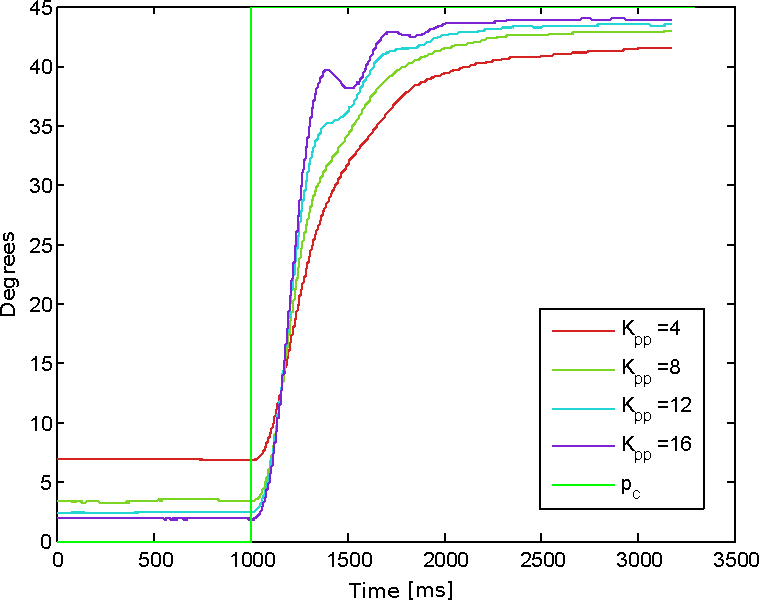
\includegraphics[width=1\textwidth,trim={0cm 0cm 0cm 0cm},clip]{figures/P2p1_K_pp_label.pdf}
	\caption{Pitch response with PD control}
\label{fig:P2p1_K_pp}
\end{figure}
\begin{figure}[!!ht!!!!!!!!tb!!]
	\centering
		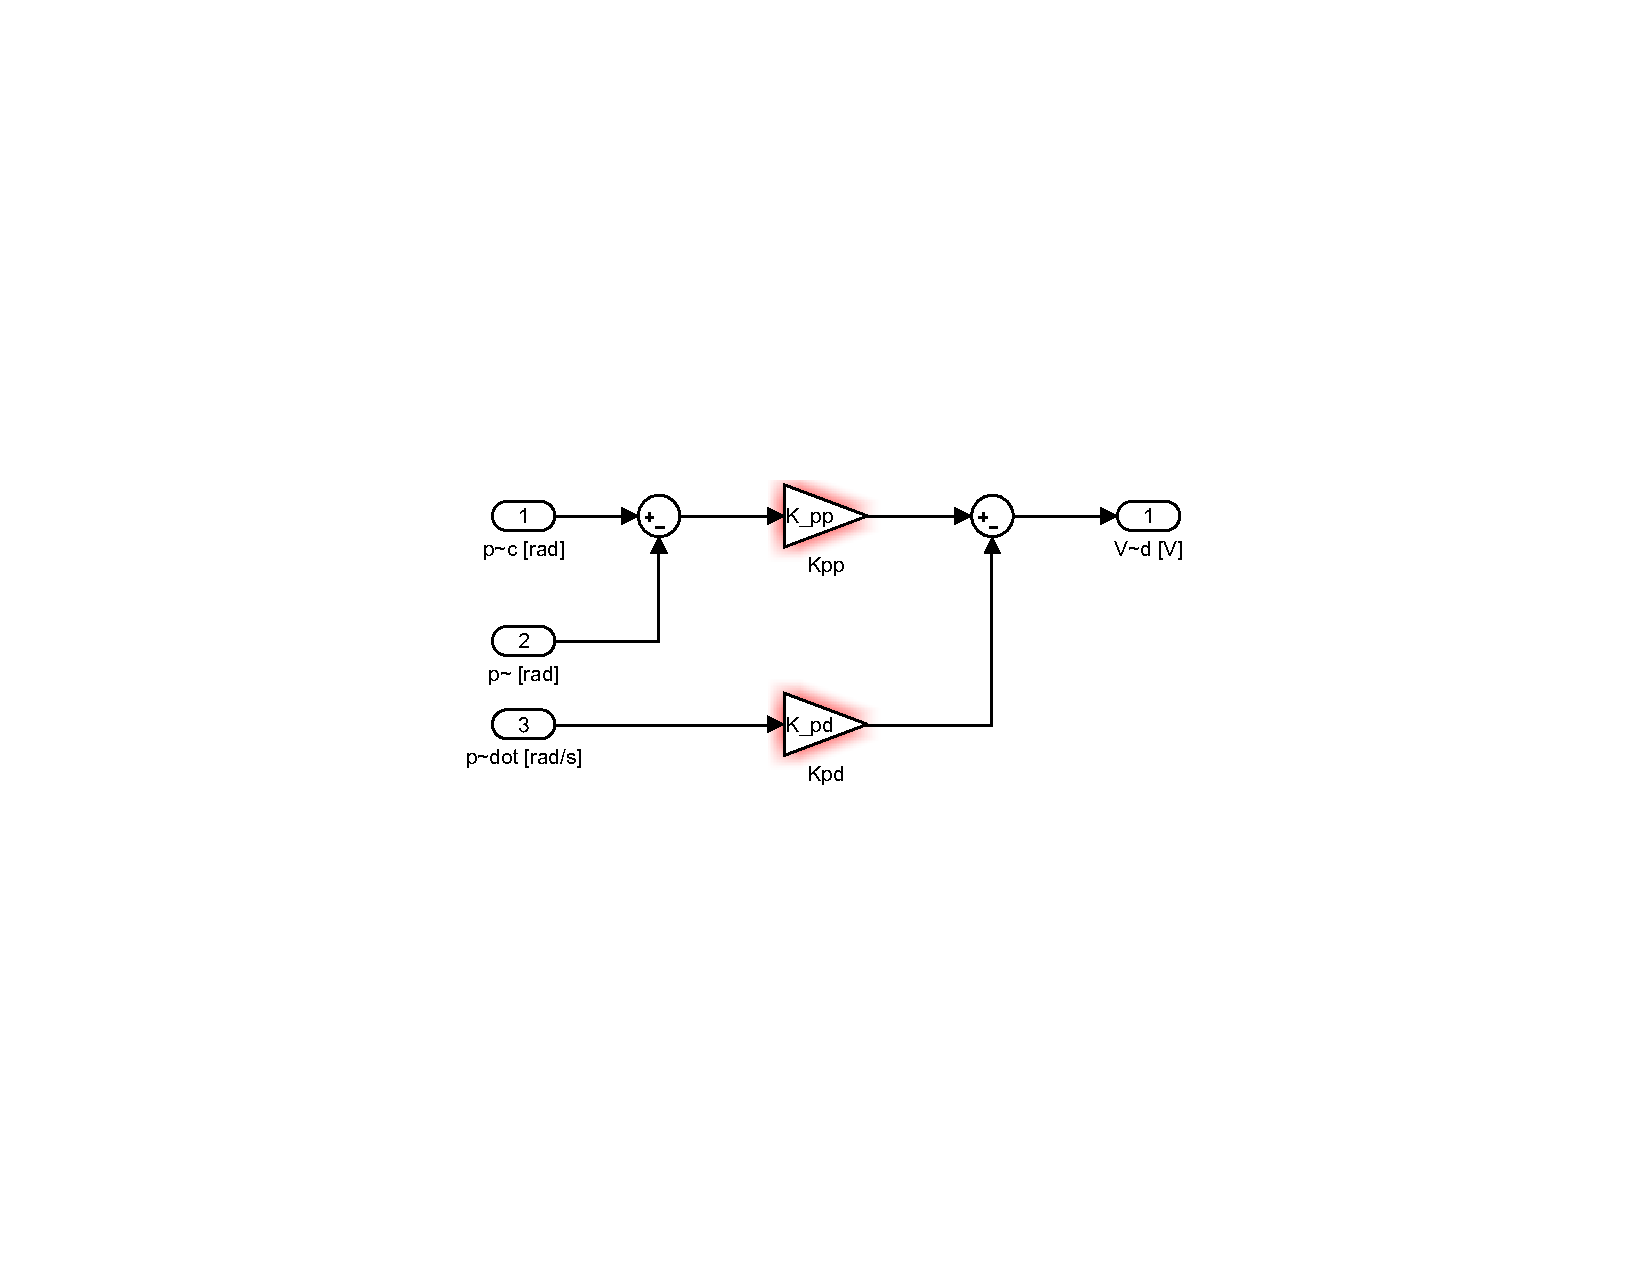
\includegraphics[scale=0.9, trim={6.2cm 8cm 0cm 4cm},clip]{figures/simulink/PD_controller.pdf}
	\caption{Inside the Pitch controller}
\label{fig:P2p1_controller}
\end{figure}
\clearpage

\subsubsection{Problem 2}
The transfer function for the travel controller in \cref{eq:P2_P} can be written as
\begin{equation}
    \frac{\td{\lambda}(s)}{\td{\lambda}_c(s)} = \frac{\rho}{s + \rho}, 
    \label{eq:P2_p_trasfer}
\end{equation}
where $\rho$ is a constant. Assuming that the pitch angle is controlled perfectly, this can be shown by rewriting \cref{eq:P1_linearised_equation_of_motion_lambda_ddot} so that
\begin{align}
    \tilde{p} &= \frac{\tdd{\lambda}}{K_3} \label{eq:P2_p_to_lambda}.
\end{align}
Inserting this into \cref{eq:P2_P} then yields
\begin{align*}
    \tdd{\lambda} &= K_3 K_{lp} (\td{\lambda}_c - \td{\lambda}),
\end{align*}
which in the laplace domain is
\begin{align*}
    s\td{\lambda} &= K_3 K_{lp} (\td{\lambda}_c - \td{\lambda}).
\end{align*}
Finally, by rearranging the terms, the transfer function becomes 
\begin{align}
    h(s) = \frac{\td{\lambda}}{\td{\lambda}_c} = \frac{K_3 K_{lp}}{s + K_3 K_{lp}},
\end{align}
which when letting $\rho = K_3 K_{lp}$ is the same as \cref{eq:P2_p_trasfer}.

To find a proper value for $K_{lp}$ one can look at the poles for both the pitch and travel controller. Because travel is dependant on pitch, pitch control should be faster than travel. From the perspective of pole placement, this means that the magnitude of the pitch poles should be greater than the travel poles.
After some trial and error, $K_{lp} = -1.15$ was found to produce a rapid response without any considerable overshoot, as can be seen in figure \cref{fig:P2p2_K_lp}. From the pole plot in figure \cref{fig:P2p2_poles} we can see that the pitch controller is much faster.
\begin{figure}[!!ht!!!!!!!!tb!!]
    \begin{minipage}{0.5\textwidth}
    	\centering
		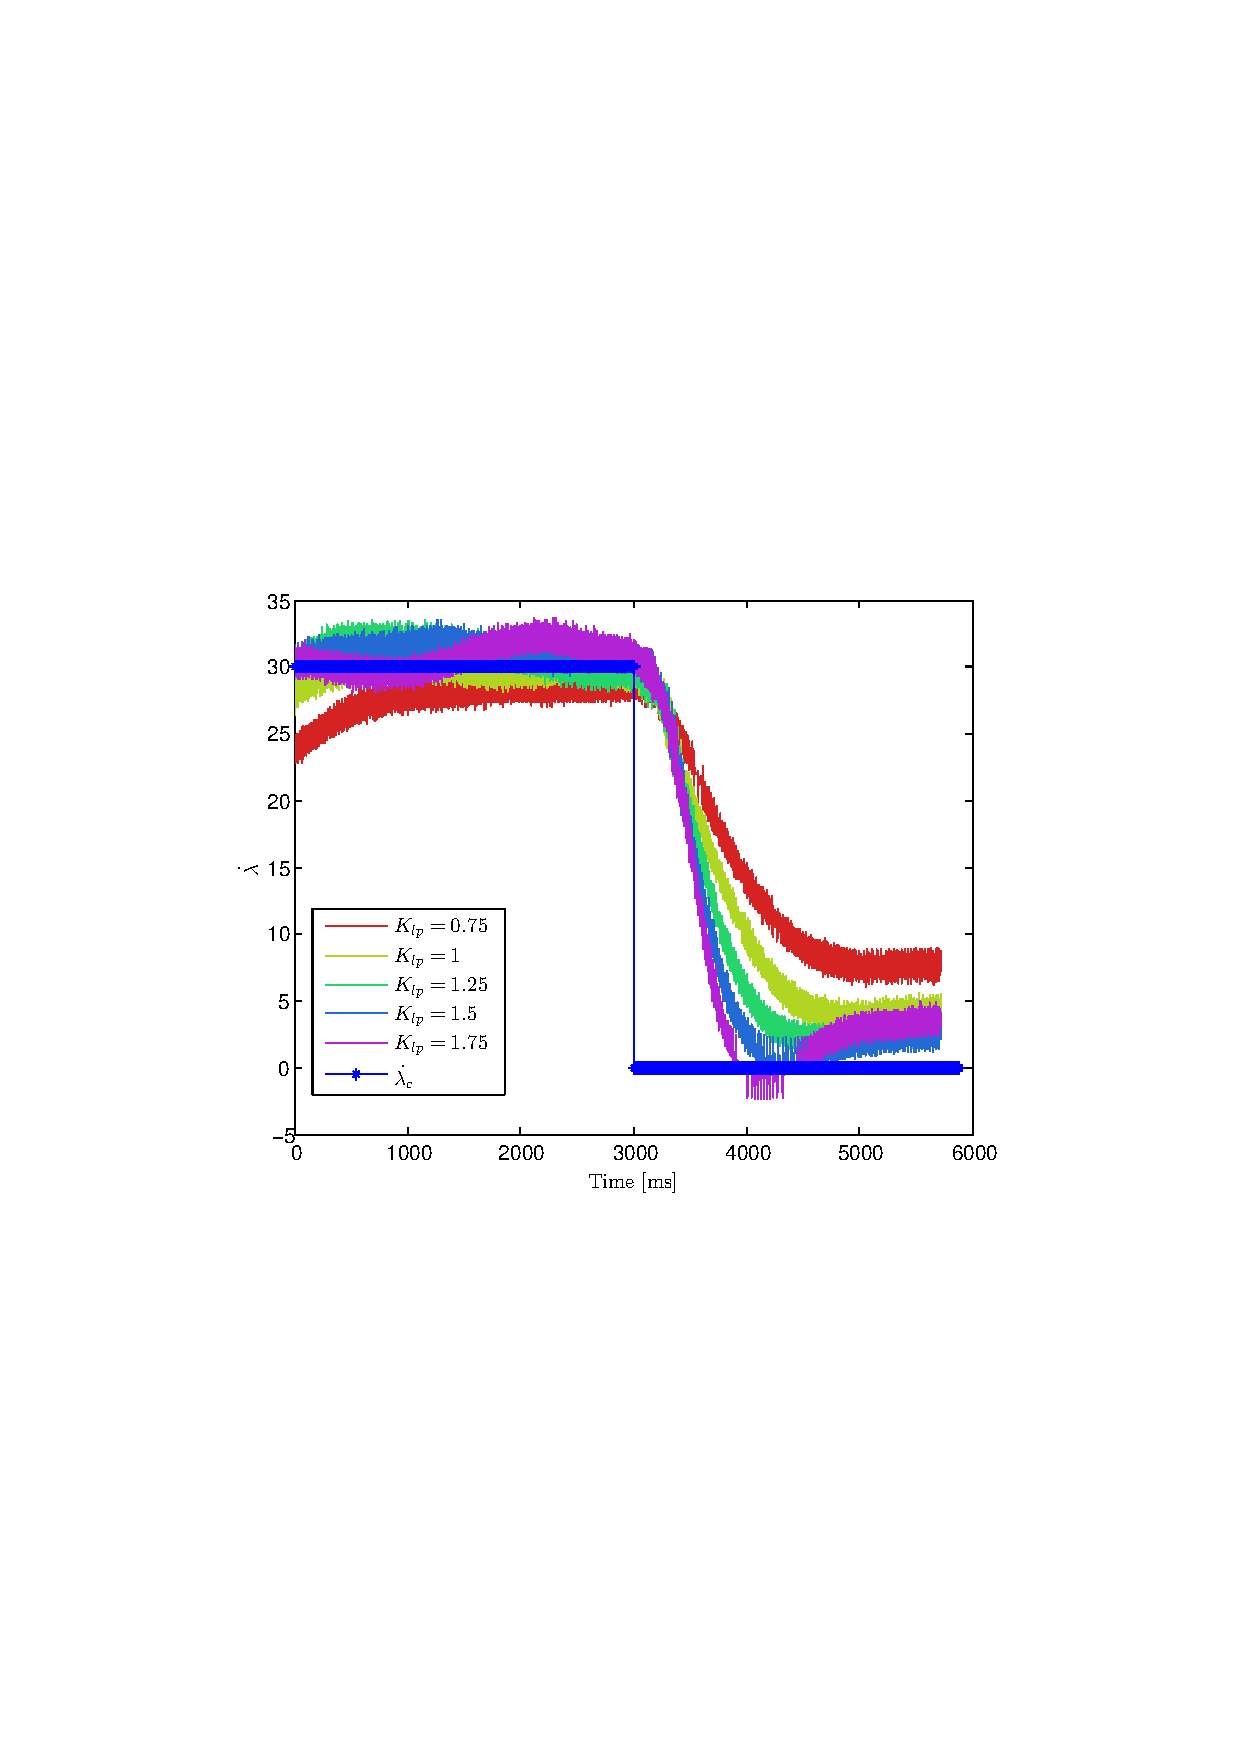
\includegraphics[width=1\textwidth,trim={4cm 9cm 4cm 9cm},clip]{figures/P2p2_Klp.pdf}
    	\caption{Travel response with P control}
	\end{minipage}
	\begin{minipage}{0.5\textwidth}
    	\centering
		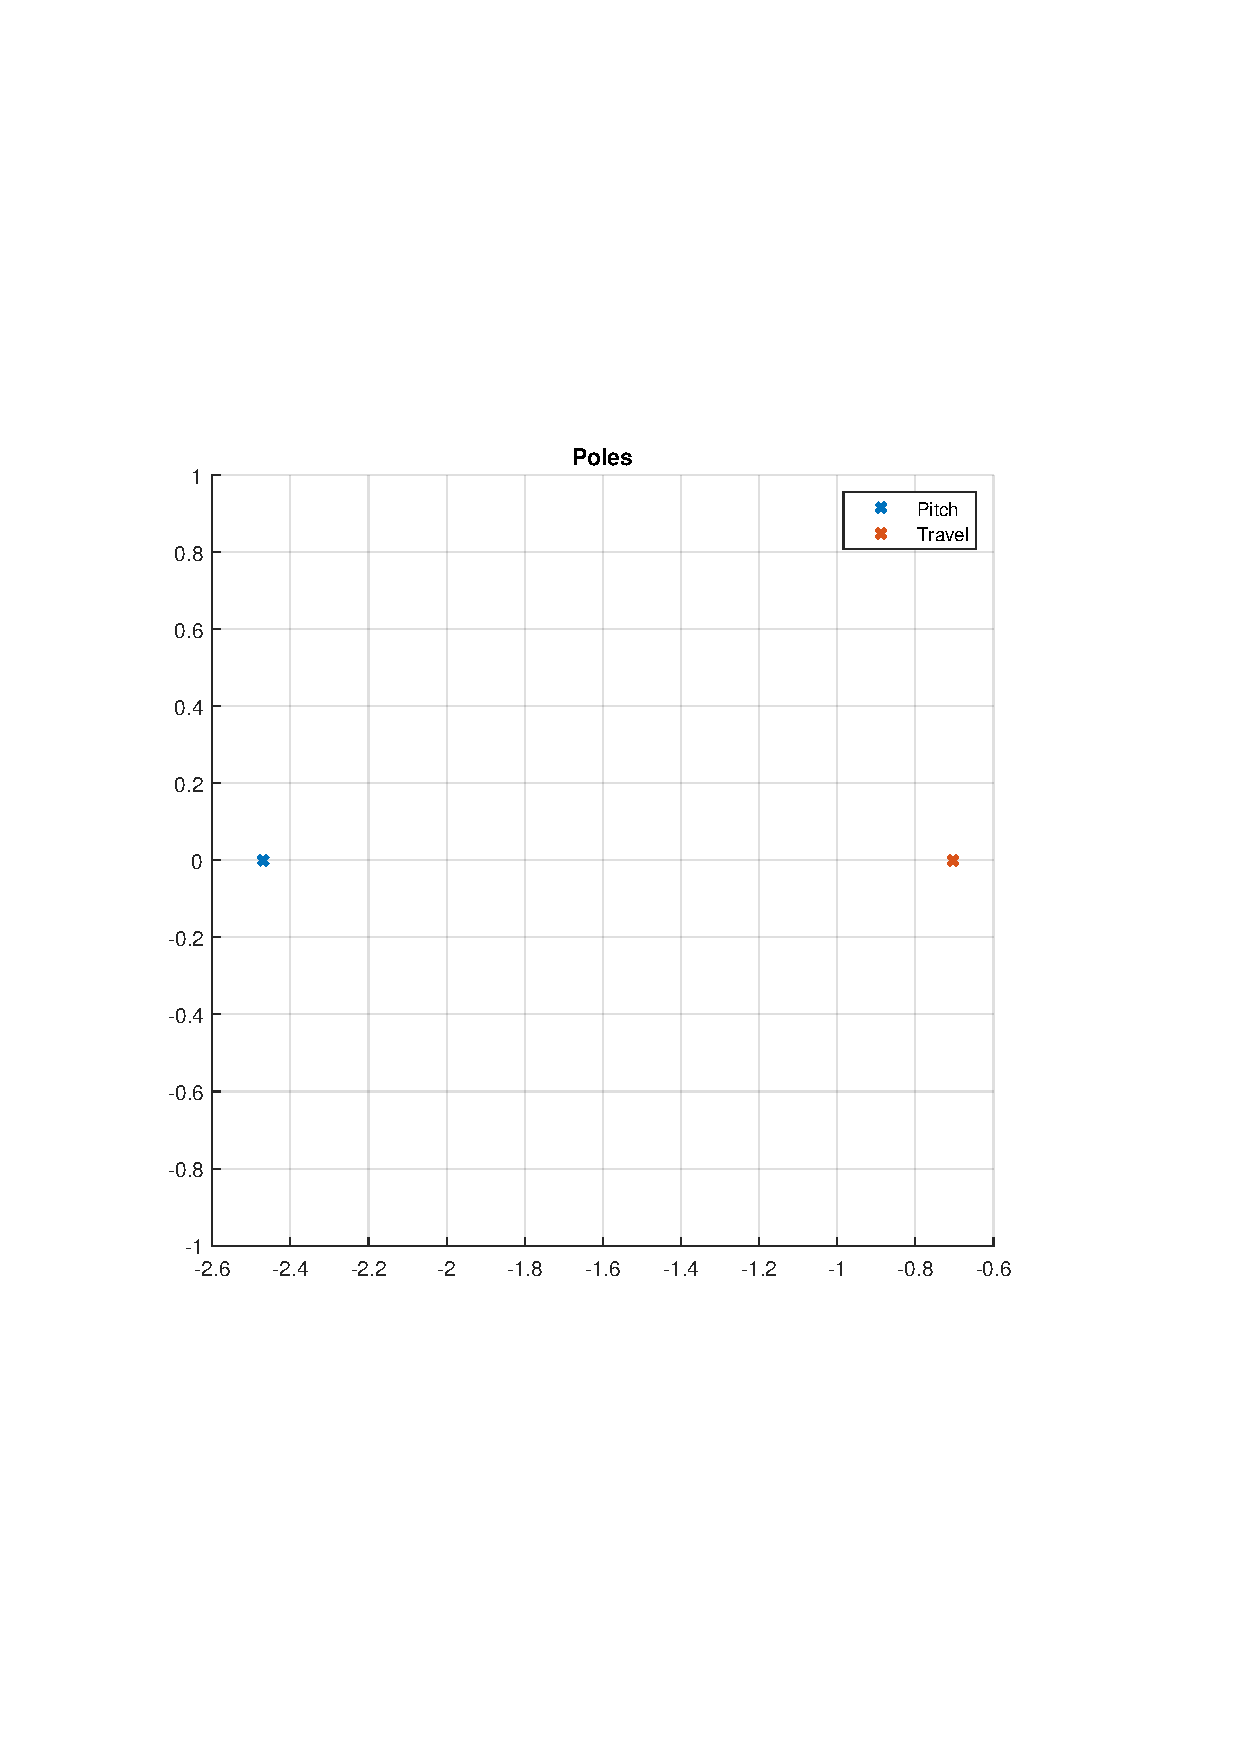
\includegraphics[width=1\textwidth,trim={2cm 7cm 3cm 6cm},clip]{figures/Travel_controller.pdf}
    	\caption{Travel and pitch controller poles}
	\end{minipage}
\label{fig:P2p2_poles}
\end{figure}
\clearpage
\begin{figure}[!!ht!!!!!!!!tb!!]
    	\centering
		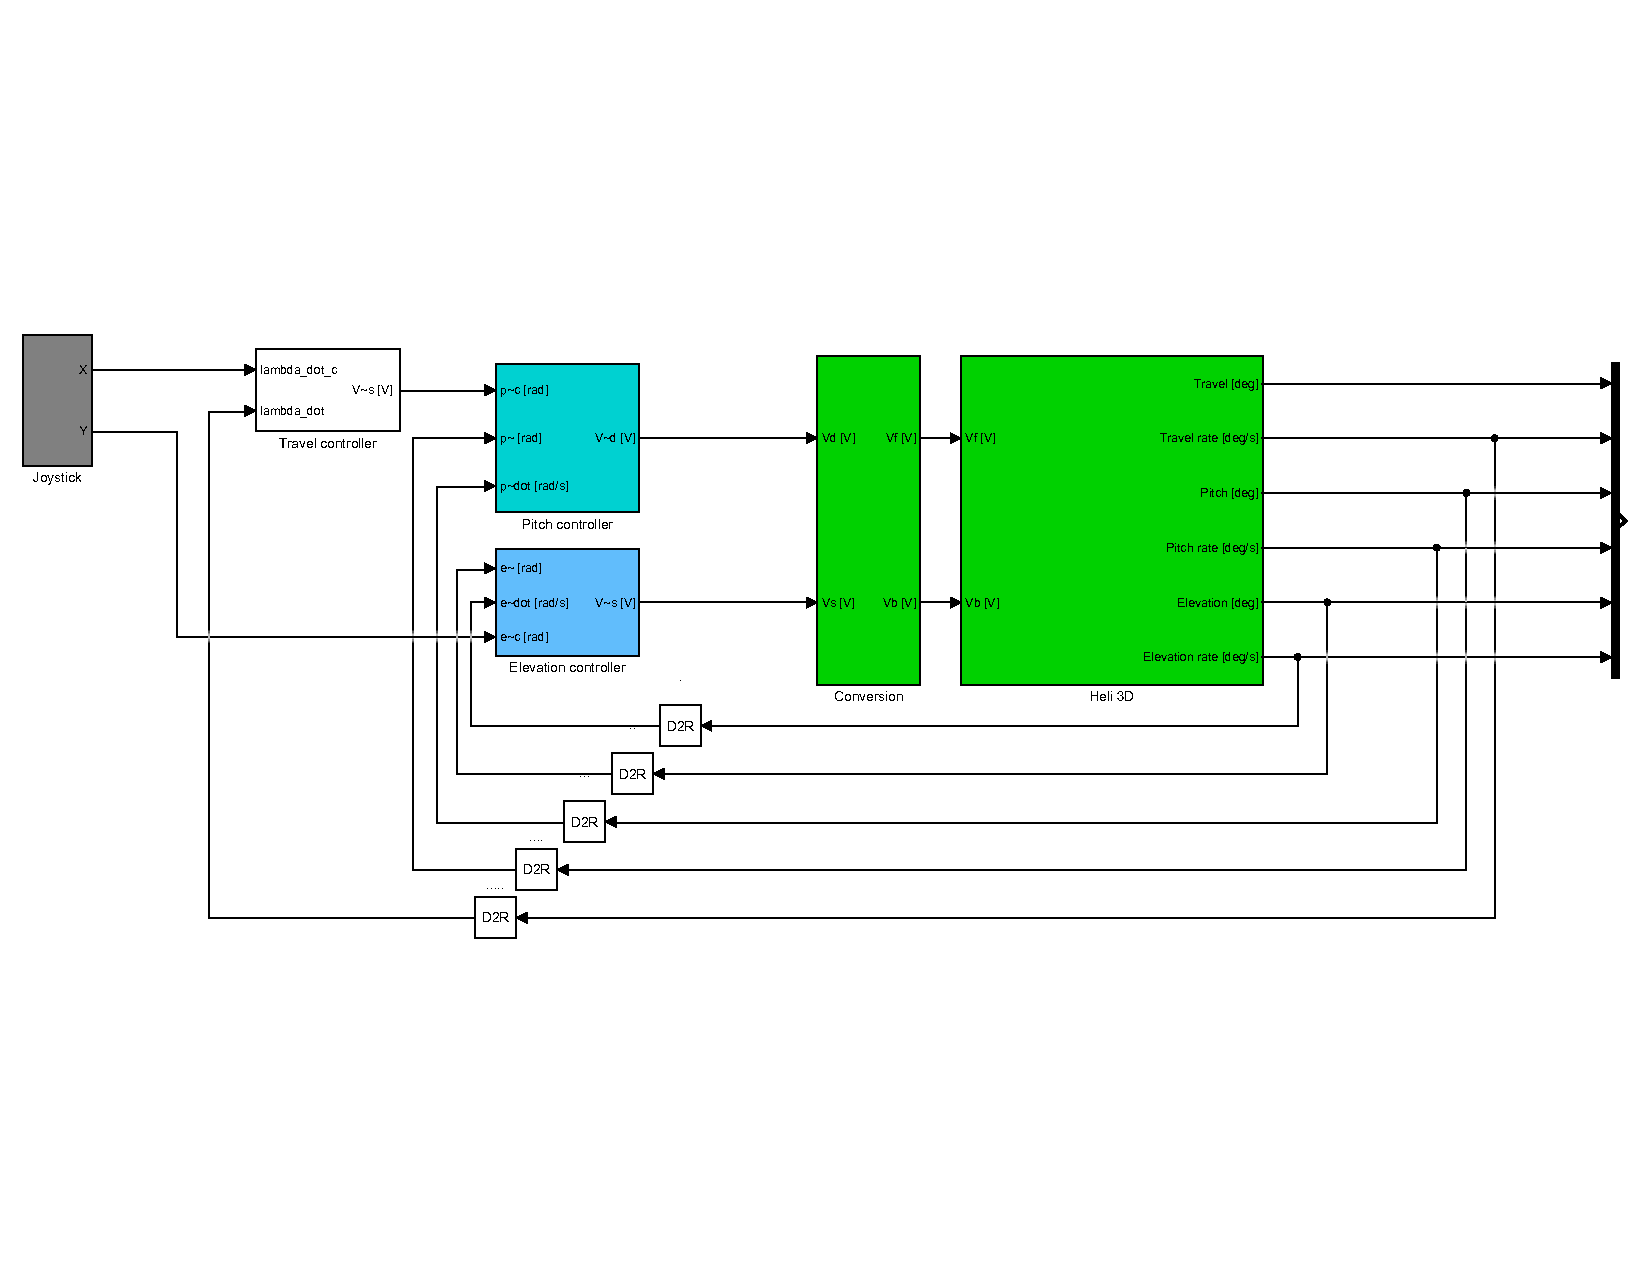
\includegraphics[width=1.1\textwidth,trim={0cm 3cm 0cm 5cm},clip]{figures/simulink/P2p2.pdf}
    	\caption{Simulink model of Part 2 problem 2}
\label{fig:P2p2_system}
\end{figure}
\begin{figure}[!!ht!!!!!!!!tb!!]
	\centering
		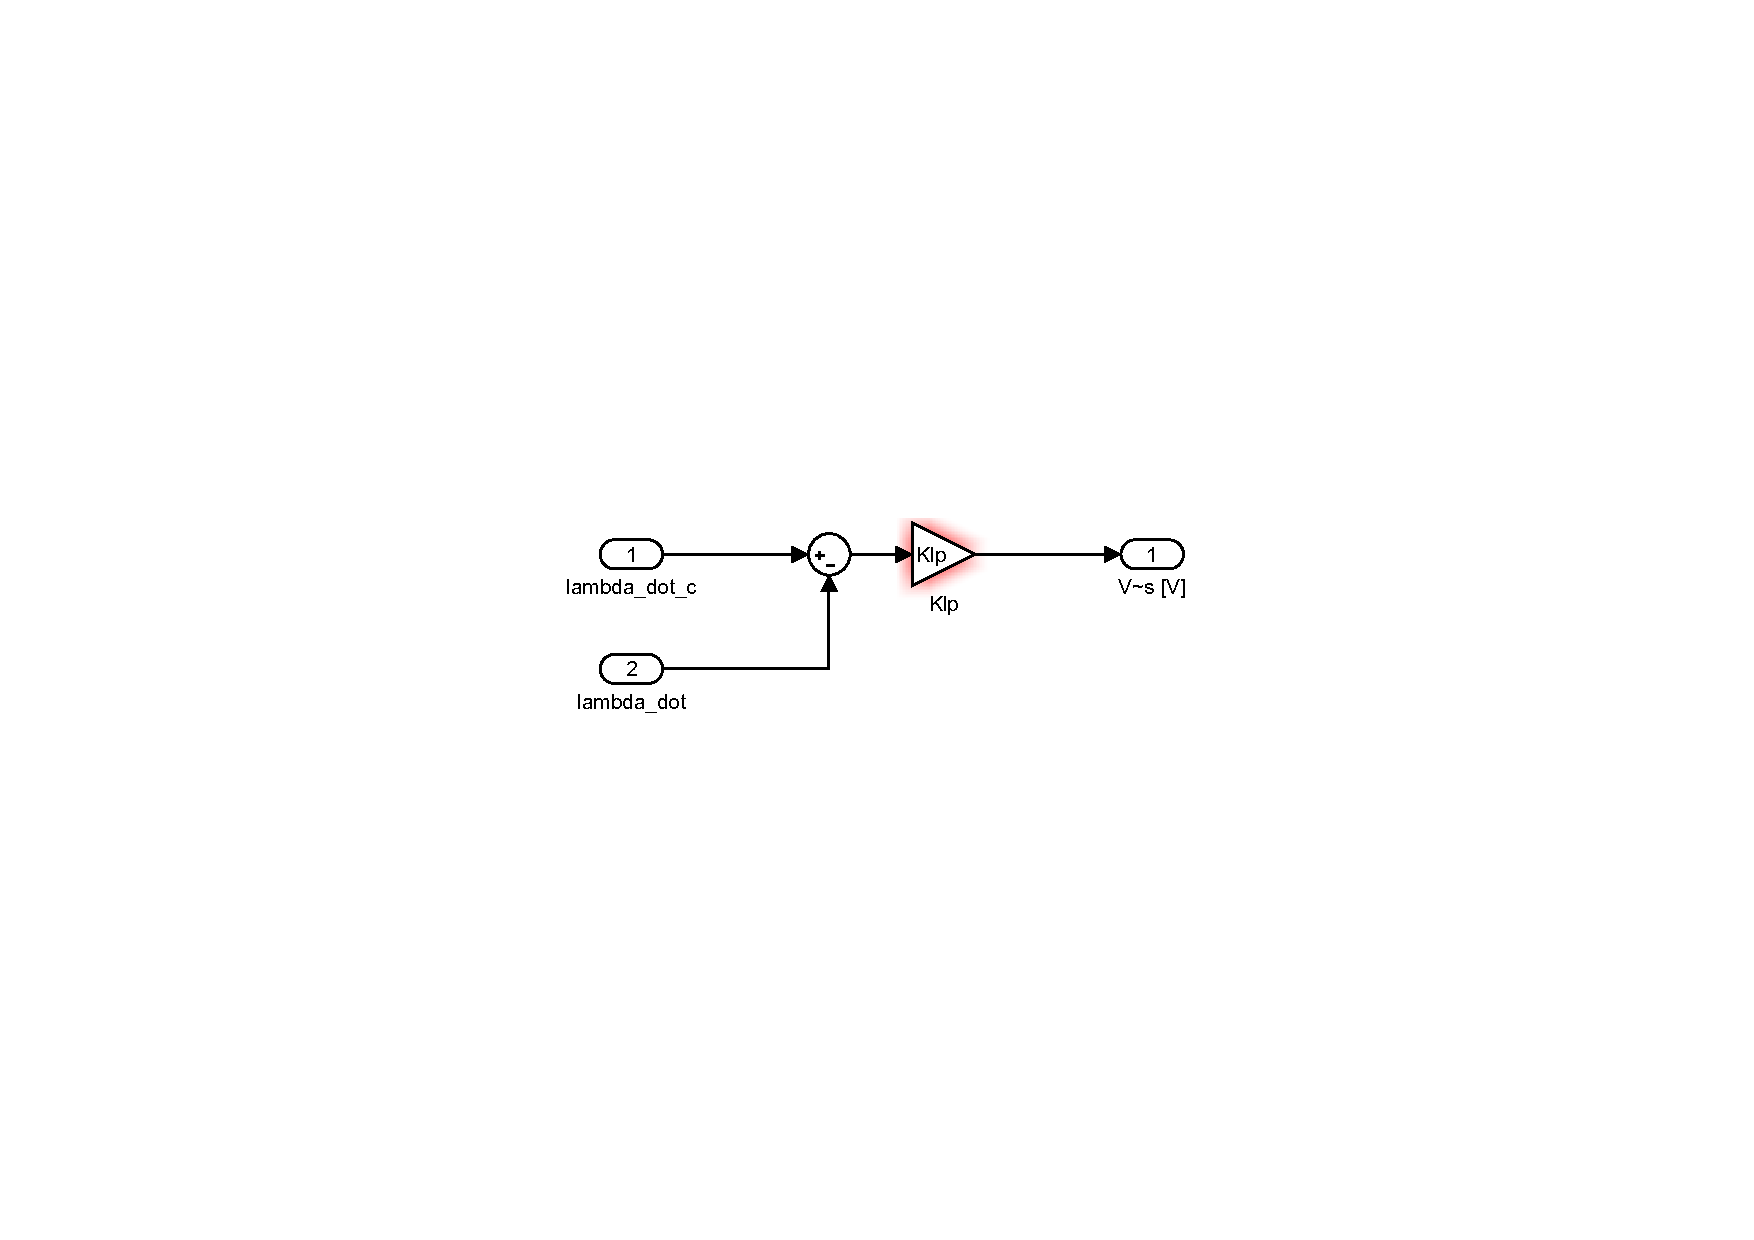
\includegraphics[scale=1.1, trim={9.2cm 8cm 0cm 4cm},clip]{figures/simulink/P_controller.pdf}
	\caption{Inside the Travel controller}
\label{fig:P2p2_controller}
\end{figure}
\clearpage

% Part III

%%%%%%%%%%%%%%%%%%%%%%%%%%%%%%%%%%%%%%%%%%%%%%%%%%%%%%%%%%%%%%%%%%%%

\subsection{Part III - Multivariable control}\label{subsec:part3}
\subsubsection{Problem 1}

Considering the linearised system in \cref{eq:P1_linearised_equations_of_motion} with a state and input vector of  

\begin{equation}\label{eq:P3_state_vector_and_input}
    \mathbf{x}=
    \begin{bmatrix}
        \tilde{p}\\
        \td{p}\\
        \td{e}
    \end{bmatrix}
    \quad\text{and}\quad
    \mathbf{u}=
    \begin{bmatrix}
        \tilde{V_s}\\
        \tilde{V_d}
    \end{bmatrix}
\end{equation}
and a state-space formulation of the form
\begin{equation}\label{eq:P3_state_space_equation}
    \dot{\mathbf{x}}=\mathbf{Ax}+\mathbf{Bu},
\end{equation}
the matrices $\mathbf{A}$ and $\mathbf{B}$ become 
\begin{subequations}\label{eq:P3_p1_A_B}
    \begin{align}
        \mathbf{A}&=
            \begin{bmatrix}
                0&1&0\\
                0&0&0\\
                0&0&0
            \end{bmatrix}\label{eq:P3_p1_A} \\
        \mathbf{B}&=
            \begin{bmatrix}
                0&0\\
                K_1&0\\
                0&K_2
            \end{bmatrix}\label{eq:P3_p1_B}.
    \end{align}
\end{subequations}
\clearpage
%%%%%%%%%%%%%%%%%%%%%%%%%%%%%%%%%%%%%%%%%%%%%%%%%%%%%%%%%%%%%%%%%%%%

\subsubsection{Problem 2}
In this problem, the purpose was to track a multivariable reference
\begin{equation}\label{eq:P3_p2_reference}
    \mathbf{r}=
        \begin{bmatrix}
            \tilde{p_c}\\
            \dot{\tilde{e_c}}
        \end{bmatrix}.
\end{equation}
Firstly, the controllability of the system is examined. Due to \cref{eq:P3_state_vector_and_input} having three states, the controllability matrix is given by
\begin{equation}\label{eq:P3_p2_controllability_matrix}
    \mathcal{C}=
        \begin{bmatrix}
            \mathbf{B}&\mathbf{AB}&\mathbf{A^2B}
        \end{bmatrix}
        =
        \begin{bmatrix}
            0   &   0   &  K_1 &0&0&0 \\
            K_1 &   0   &  0   &0&0&0 \\
            0   &   K_2 &  0   &0&0&0
        \end{bmatrix}.
\end{equation}
With the values $K_1=0.9046$ and $K_2=0.1555$ inserted, this becomes 
\begin{equation}
    \mathcal{C}=
        \begin{bmatrix}
            0      &   0      &  0.9046 &0&0&0 \\
            0.9046 &   0      &  0      &0&0&0 \\
            0      &   0.1555 &  0      &0&0&0
        \end{bmatrix}.
\end{equation}
\begin{figure}[!!ht!!!!!!!!tb!!]
	\centering
		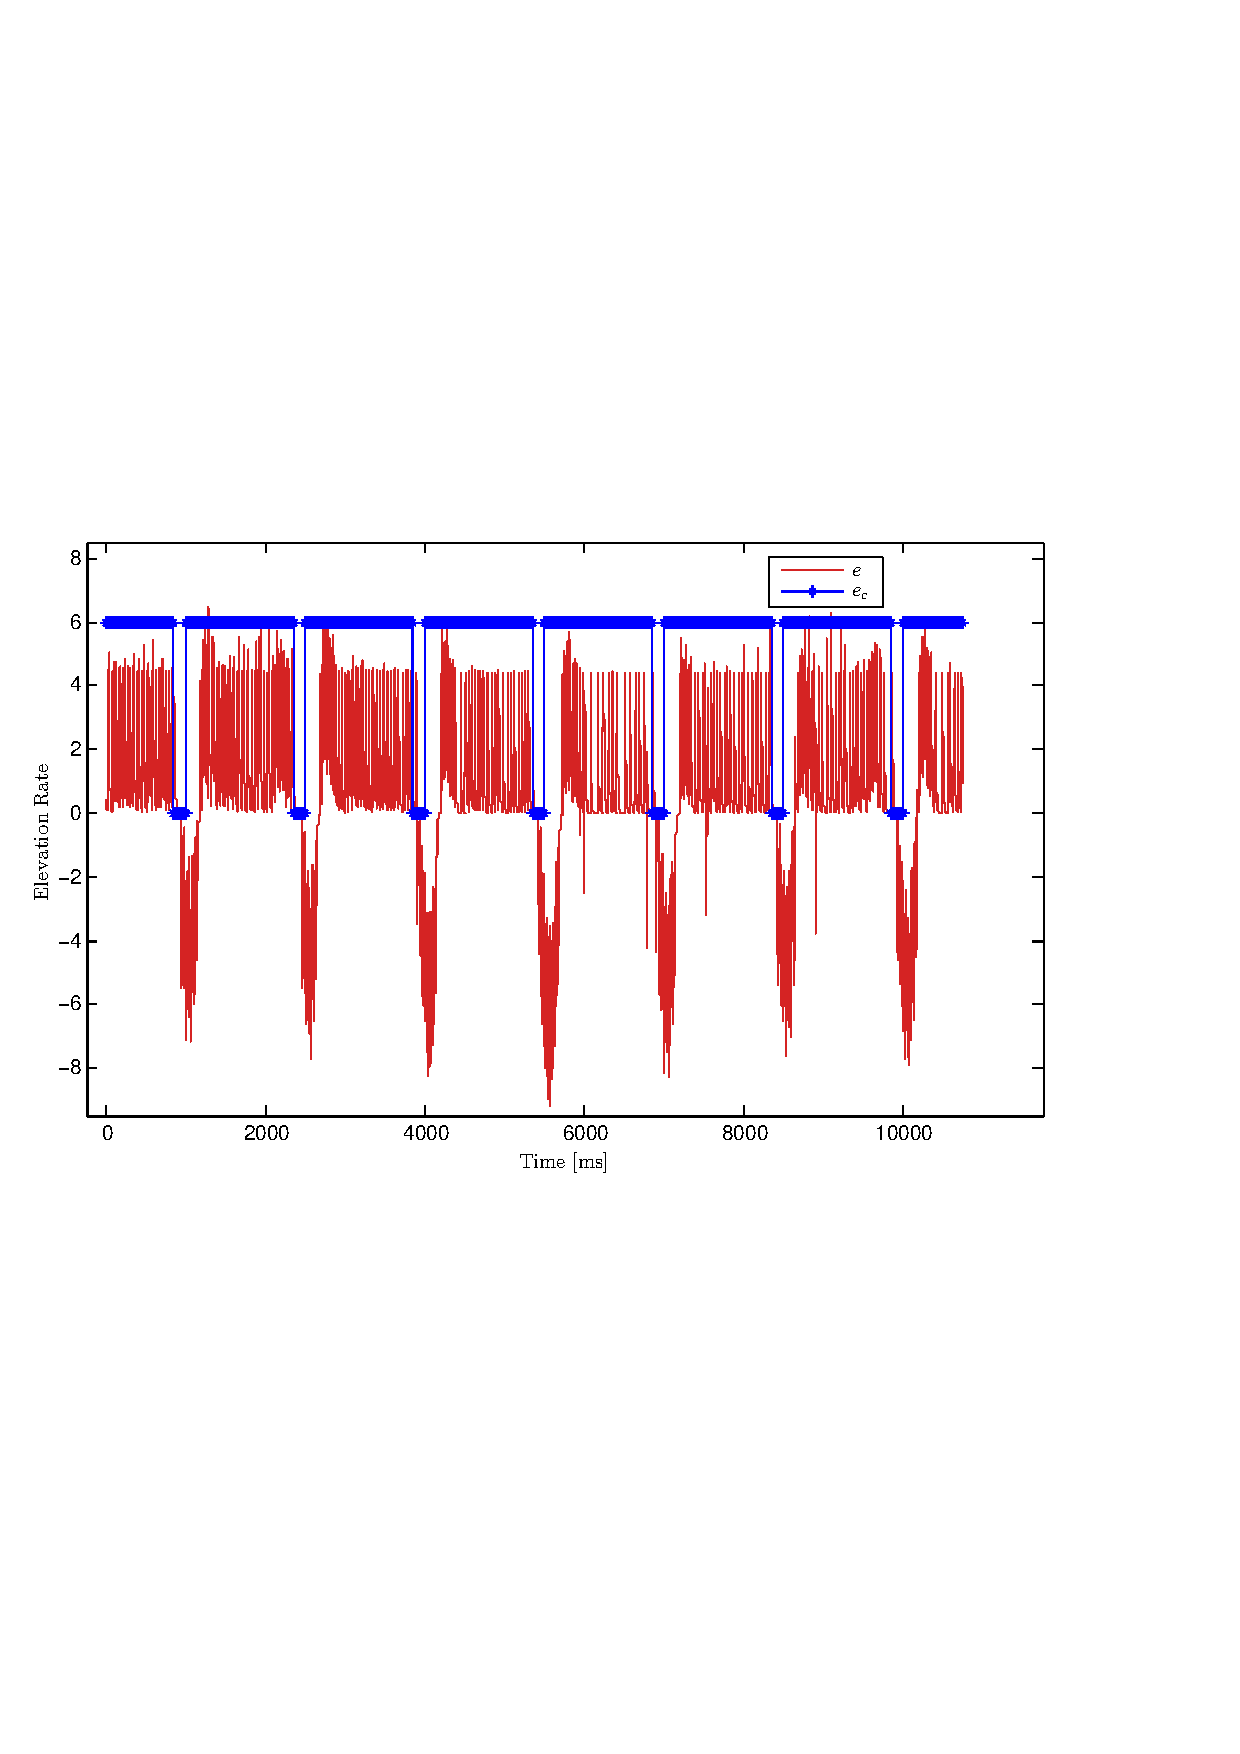
\includegraphics[width=1\textwidth,trim={4cm 9cm 4cm 9cm},clip]{figures/P3p2_e_dot.pdf}
	\caption{Travel response with P control}
\label{fig:P3p2_e_dot}
\end{figure}
\clearpage
\begin{figure}[!!ht!!!!!!!!tb!!]
	\centering
		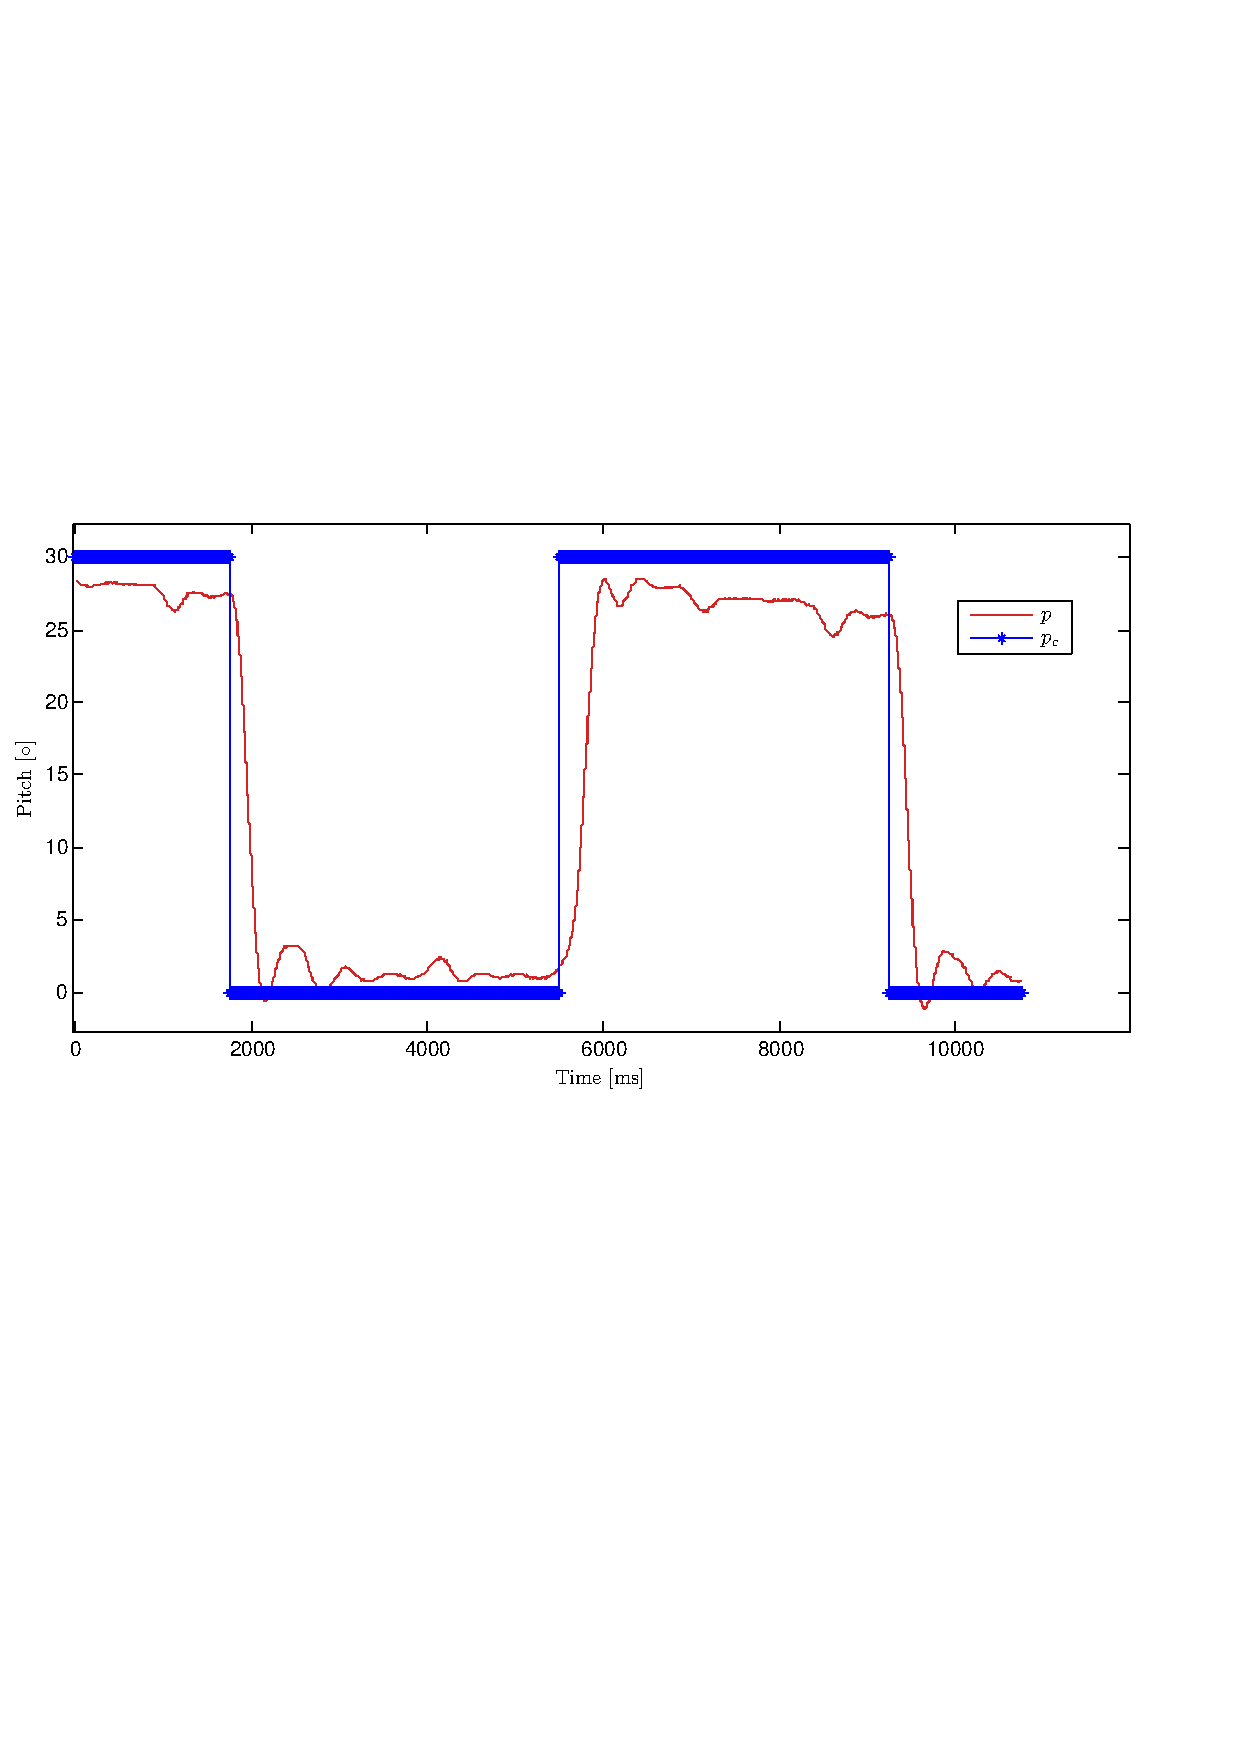
\includegraphics[width=1\textwidth,trim={4cm 9cm 4cm 9cm},clip]{figures/P3p2_p.pdf}
	\caption{Travel response with P control}
\label{fig:P3p2_p}
\end{figure}
\clearpage

There is no need for feed forward gain when using integral effect. So we can use the same P matrix as in the previous problem.\cite{Chen2014}


% Part IV

%%%%%%%%%%%%%%%%%%%%%%%%%%%%%%%%%%%%%%%%%%%%%%%%%%%%%%%%%%%%%%%%%%%%

\subsection{Part IV - State estimation}\label{subsec:part4}
\subsubsection{Problem 1}
The system given in \cref{eq:P1_linearised_equations_of_motion} can be expressed as a state space representation with the vectors
\begin{align}
    \textbf{x} = \begin{bmatrix}
        \tilde p        \\
        \td p           \\
        \tilde e        \\
        \td e           \\
        \tilde \lambda  \\
        \td \lambda
    \end{bmatrix}, \hspace{0.5cm}
    \mathbf{u} = \begin{bmatrix}
        \tilde V_s \\
        \tilde V_d
    \end{bmatrix} \hspace{0.5cm} \text{and} \hspace{0.5cm}
    \textbf{y} = \begin{bmatrix}
        \tilde p        \\
        \tilde e        \\
        \tilde \lambda  \\
    \end{bmatrix}.
\end{align}
The system can thus be expressed on the form
\begin{align}
    \mathbf{\dot x} &= \mathbf{Ax} + \mathbf{B} \\
    \mathbf{y} &= \mathbf{Cx},
\end{align}
with the matrices
\begin{equation}
    \setstackgap{L}{1.1\baselineskip}
    \fixTABwidth{T}
    \label{p4_sys_AB}
    \mathbf A = 
    \bracketMatrixstack{
		0   & 1 & 0 & 0 & 0 & 0 \\
		0   & 0 & 0 & 0 & 0 & 0 \\
		0   & 0 & 0 & 1 & 0 & 0 \\
		0   & 0 & 0 & 0 & 0 & 0 \\
		0   & 0 & 0 & 0 & 0 & 1 \\
		K_3 & 0 & 0 & 0 & 0 & 0 
	}
	\text{,}
	\hspace{0.5cm}
	\mathbf B = 
	\bracketMatrixstack{
	    0   & 0   \\
	    0   & K_1 \\
	    0   & 0 & \\
	    K_2 & 0   \\
	    0   & 0   \\
	    0   & 0
	}
\end{equation}
and
\begin{equation}
    \label{p4_sys_C}
    \mathbf C = 
    \begin{bmatrix}
        1   &   0   &   0   &   0   &   0   &   0 \\
        0   &   0   &   1   &   0   &   0   &   0 \\
        0   &   0   &   0   &   0   &   1   &   0
    \end{bmatrix}.
\end{equation}
\subsubsection{Problem 2}
\textbf{Observability Analysis}\\
From the system matrix in \eqref{p4_sys_AB} and the output matrix in \eqref{p4_sys_C}, the observability matrix can be found to be
\begin{equation}
    \setstackgap{L}{1.1\baselineskip}
    \fixTABwidth{T}
    \mathbf{\mathcal{O}} = 
        \begin{bmatrix}
        \mathbf{C}      \\
        \mathbf{CA}     \\
        \mathbf{CA^2}   \\
        \mathbf{CA^3}   \\
        \mathbf{CA^4}   \\
        \mathbf{CA^5}   \\
    \end{bmatrix}
    =
    \bracketMatrixstack{
    1       & 0       & 0 & 0 & 0 & 0 \\
    0       & 0       & 1 & 0 & 0 & 0 \\
    0       & 0       & 0 & 0 & 1 & 0 \\
    0       & 1       & 0 & 1 & 0 & 0 \\
    0       & 0       & 0 & 0 & 0 & 1 \\
    0       & 0       & 0 & 0 & 0 & 0 \\
    0       & 0       & 0 & 0 & 0 & 0 \\
    -0.612  & 0       & 0 & 0 & 0 & 0 \\
    0       & 0       & 0 & 0 & 0 & 0 \\
    0       & 0       & 0 & 0 & 0 & 0 \\
    0       & -0.612  & 0 & 0 & 0 & 0 \\
    0       & 0       & 0 & 0 & 0 & 0 \\
    0       & 0       & 0 & 0 & 0 & 0 \\
    0       & 0       & 0 & 0 & 0 & 0 \\
    0       & 0       & 0 & 0 & 0 & 0 \\
    0       & 0       & 0 & 0 & 0 & 0 \\
    0       & 0       & 0 & 0 & 0 & 0 }
    \text{.}
\end{equation}
The matrix has full column rank, which means the system is observable.\\\\
\textbf{Linear Observer Design}\\
We wish to control the system using an estimated state $\mathbf{\hat{x}}$. A \textit{linear observer} (or closed-loop estimator) is then
\begin{equation}
    \label{eq:observer}
    \mathbf{\dot{\hat{x}}} = \mathbf{A\hat{x}} + \mathbf{Bu} + \mathbf{L} (\mathbf{y} - \mathbf{C\hat{x}}),
\end{equation}
where $\mathbf A$, $\mathbf B$ and $\mathbf C$ are as before and $\mathbf L$ is the \textit{observer gain matrix}. \\
Replacing the output with $\mathbf{C}\mathbf{x}$ and rearranging yields
\begin{equation*}
   \mathbf{\dot{\hat{x}}} = (\mathbf{A} - \mathbf{LC})(\mathbf{\hat{x}} - \mathbf{x}) + \mathbf{Ax} + \mathbf{LC}(\mathbf{x} - \mathbf{\hat{x}}),
\end{equation*}
and when inserting the estimation error (denoted $\mathbf{d}$ as in \textit{deviation} here, to not confuse it with the elevation $e$), 
\begin{equation}
    \mathbf{d} = \hat{\mathbf{x}} - \mathbf{x} \label{eq:est_error},
\end{equation}
along with its derivative, the observer's error dynamics, become
\begin{equation}
    \mathbf{\dot{d}} = (\mathbf{A} - \mathbf{LC})\mathbf{d}. \label{eq:observer_error_sys}
\end{equation}
Good state estimation is essential to properly control the helicopter. The error dynamics of the observer thus need to be faster than the dynamics of the feedback controller. This corresponds to the poles of the closed loop observer being more \textit{negative} than the controller poles. Conveniently, by theorem 8.O3 in Chen, the poles of the closed loop observer, i.e. the eigenvalues of $\mathbf{A} - \mathbf{LC}$, can be placed arbitrarily with appropriate choice of observer gain $\mathbf{L}$.\cite{Chen2014}

To place the poles like so, one can use the matlab \texttt{place} command. This command will output a feedback gain matrix that will place the poles of a closed loop system at the values given in a vector $\mathbf{p}$.
This applies to using a feedback controller such as $\mathbf{u} = -\mathbf{Kx}$. In that case, the closed loop dynamics of the system, $\mathbf{\dot{x}} = \mathbf{Ax} + \mathbf{Bu}$, will be
\begin{equation*}
    \mathbf{\dot{x}} = (\mathbf{A} - \mathbf{BK})\mathbf{x}.
\end{equation*}
 Using the  matlab \texttt{place} command as such:
\begin{verbatim}
    K = place(A, B, p);
\end{verbatim}
will produce a feedback gain matrix $\mathbf{K}$, that places the eigenvalues of $\mathbf{A} - \mathbf{BK}$ at the desired values.\cite{MathWorks2018}

For the closed loop observer in \eqref{eq:observer}, the only modifiable matrix is $\mathbf{L}$. By the properties of the transpose, 
\begin{equation*}
    (\mathbf{A} - \mathbf{LC})^\text{T} = \mathbf{A}^\text{T} - (\mathbf{LC})^\text{T} = \mathbf{A}^\text{T} - \mathbf{C}^\text{T} \mathbf{L}^\text{T},
\end{equation*}
such that
\begin{equation*}
    \mathbf{L}^\text{T} = \texttt{Place}(\mathbf{A}^\text{T}, \mathbf{C}^\text{T}, \mathbf{p}).
\end{equation*}
And so finally, by the property that any matrix has eigenvalues identical to its transpose, the required matrix can be calculated as
\begin{equation}
    \label{eq:est_pole_place}
    \mathbf{L} = \texttt{Place}(\mathbf{A}^\text{T}, \mathbf{C}^\text{T}, \mathbf{p})^\text{T},
\end{equation}
where the desired eigenvalues are given in the vector $\mathbf{p}$.\\
Furthermore, by substituting the estimate $\mathbf{\hat{x}}$ for $\mathbf{x}$ in the feedback controller $\mathbf{u} = -\mathbf{Kx}$ from problem 3, the estimated system becomes
\begin{equation}
    \mathbf{\dot{\hat{x}}} = (\mathbf{A} - \mathbf{LC} - \mathbf{BK})\mathbf{\hat{x}} - \mathbf{L} \mathbf{y}.
\end{equation}
Thus, the dynamics of the closed loop system, with controller and estimator are 
\begin{align}
    \begin{bmatrix}
    \mathbf{\dot{x}} \\
        \mathbf{\dot{d}}
        \end{bmatrix}
    = \begin{bmatrix}
        \mathbf{A} - \mathbf{BK} & \mathbf{BK} \\
        \mathbf{0}               & \mathbf{A} - \mathbf{LC}
    \end{bmatrix}
    \begin{bmatrix}
        \mathbf{x} \\
        \mathbf{d}
    \end{bmatrix}.
\end{align}
Note how, since this matrix is triangular, its eigenvalues are simply those of the diagonal matrices. The stability of the entire system can hence be determined by verifying stability in the observer and the system separately,\cite{StackExchange} a principle known as the \textit{separation principle}.\cite{Chen2014}\\\\
\textbf{Observer Tuning}\\
By the separation principle, tuning of the observer can be done independently of the controller. However, as mentioned previously, the poles of the observer should be placed much further to the left in the complex plane than the poles of the closed loop feedback controller. With the \texttt{place} command, the poles are placed in a fan as illustrated in figure \ref{fig:P4p2_observer_poles}.
\begin{figure}[htb]
    \begin{minipage}{0.5\textwidth}
    	\centering
    	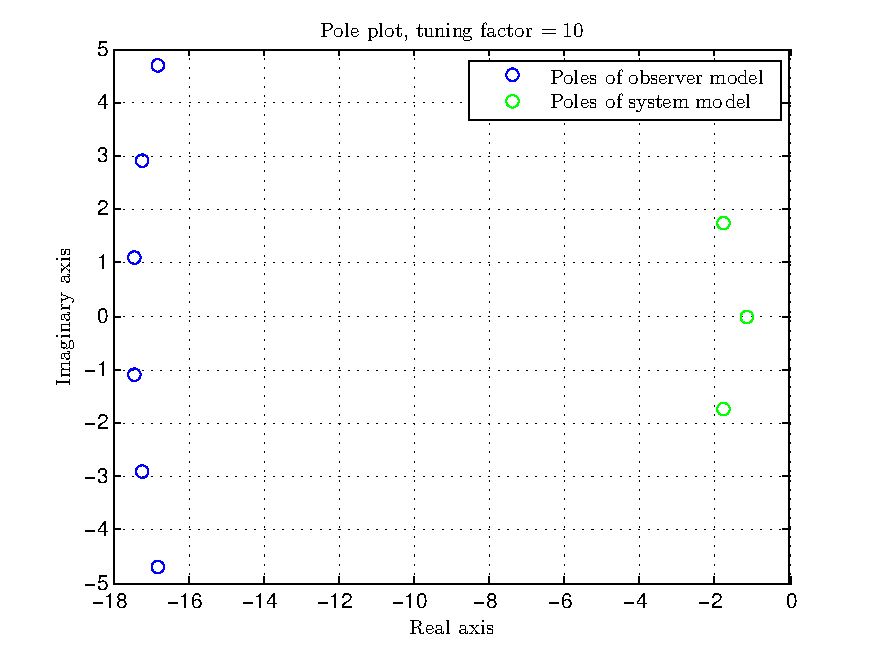
\includegraphics[width=1\textwidth,trim={0cm 0cm 0cm 0cm},clip]{figures/P4p2_pole_plot_tuning_factor_10.pdf}
    	\caption{Observer and system poles}
        \label{fig:P4p2_observer_poles}
    \end{minipage}
    \begin{minipage}{0.5\textwidth}
        \centering
    	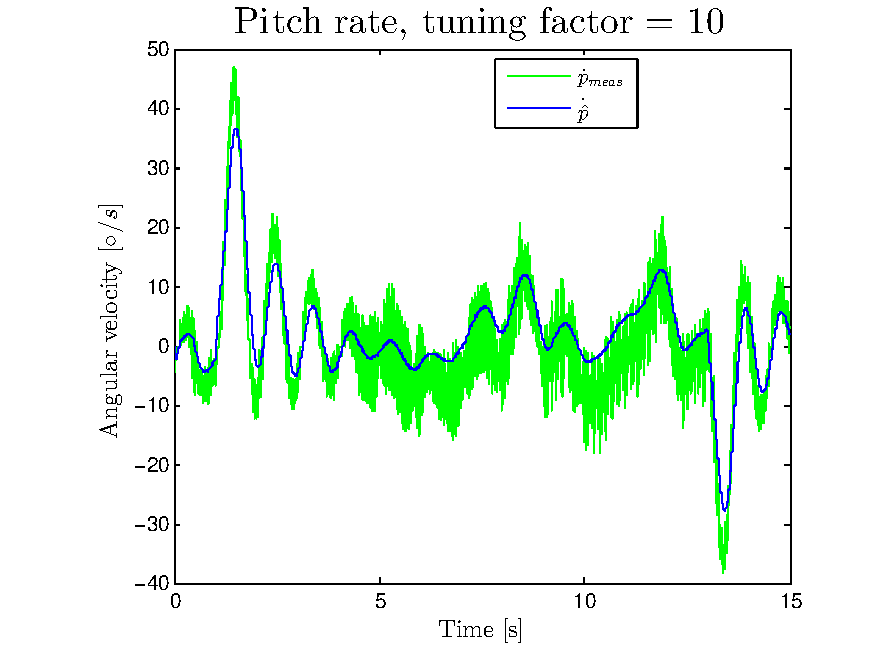
\includegraphics[width=1\textwidth,trim={0cm 0cm 0cm 0cm},clip]{figures/P4p2_pitch_rate_tuning_factor_10.pdf}.
    	\caption{Pitch rate with timid observer}
        \label{fig:P4p2_pitch_rate_10}
    \end{minipage}
\end{figure}
Having the poles be quite negative as they are here, makes the observer fast and easily able to track the state closely, neither does it introduce any noticeable lag or instability into the system.

An example plot showing the estimated pitch rate, $\dot{\hat{p}}$ (in blue) and the measured state (in green) are shown in figure \ref{fig:P4p2_pitch_rate_10}, which confirms these assumptions. The only considerable estimation error appears in the pitch rate, when the helicopter turns quickly. This is likely caused by the pitch rate being so far from zero, which is the value it was linearized around. Had the other two estimates, elevation rate and travel rate, displayed similar behaviour, estimation errors would probably appear there too. However, since the states are so much slower, this is not the case.

The poles in this case were placed around $-17$. This makes the observer fast enough for this application, but not fast enough to track the state perfectly. This slowness also has the side effect of low-pass filtering the response, which makes for clear looking plots. 

Nevertheless, it can be useful to make the poles even more negative. Placing them at around $-250$ for instance, makes the response very noisy, but with very close tracking of the actual state, as can be shown in figure \ref{fig:P4p2_travel_rate_150}.

\begin{figure}[htb]
	\centering
		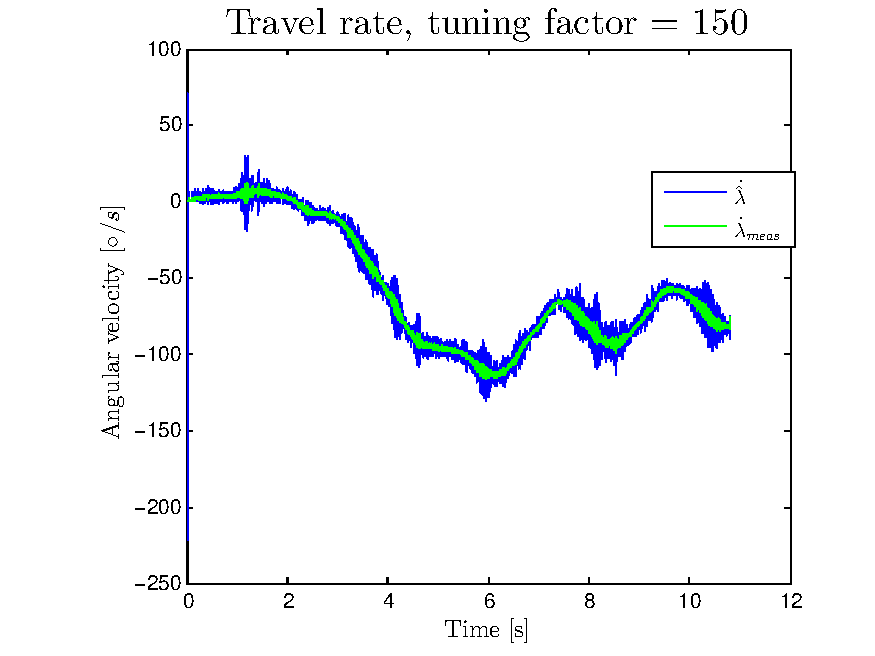
\includegraphics[width=0.6\textwidth,trim={0cm 0cm 0cm 0cm},clip]{figures/P4p2_travel_rate_tuning_factor_150_OLD.pdf}.
	\caption{Travel rate with very fast observer}
\label{fig:P4p2_travel_rate_150}
\end{figure}
It is in fact easy to show that very negative eigenvalues of $\mathbf{L}$ scale up any unwanted measurement measurement noise heavily, just like in this case. Rewriting \eqref{eq:observer} with $\mathbf{y} = \mathbf{Cx} + \mathbf{w}$ as output, where the vector $\mathbf{w}$ represents the measurement noise in the output, means \eqref{eq:observer_error_sys} instead becomes
\begin{equation}
    \mathbf{\dot{d}} = (\mathbf{A} - \mathbf{LC})\mathbf{d} - \mathbf{Lw}.
\end{equation}
An $\mathbf{L}$ matrix with very negative eigenvalues will thus result in $|\mathbf{Lw}|$ becoming very large and introduce high amplitude noise into the estimation error dynamics. 

A middle ground, with poles placed around $-120$, results in precise estimation of the measured value. It introduces a bit of noise, but no more than their measured counterparts do. Plots that show how well the estimated states, $\dot{\hat{p}}$, $\dot{\hat{e}}$ and $\dot{\hat{\lambda}}$ compare to the measured states, are shown in figures \ref{fig:P4p2_pitch_rate_70}, \ref{fig:P4p2_elevation_rate_70} and \ref{fig:P4p2_travel_rate_70}, respectively. The pole placement is shown in figure \ref{fig:P4p2_pole_plot_70} 
\begin{figure}[htb]
    \begin{minipage}{0.5\textwidth}
    	\centering
    	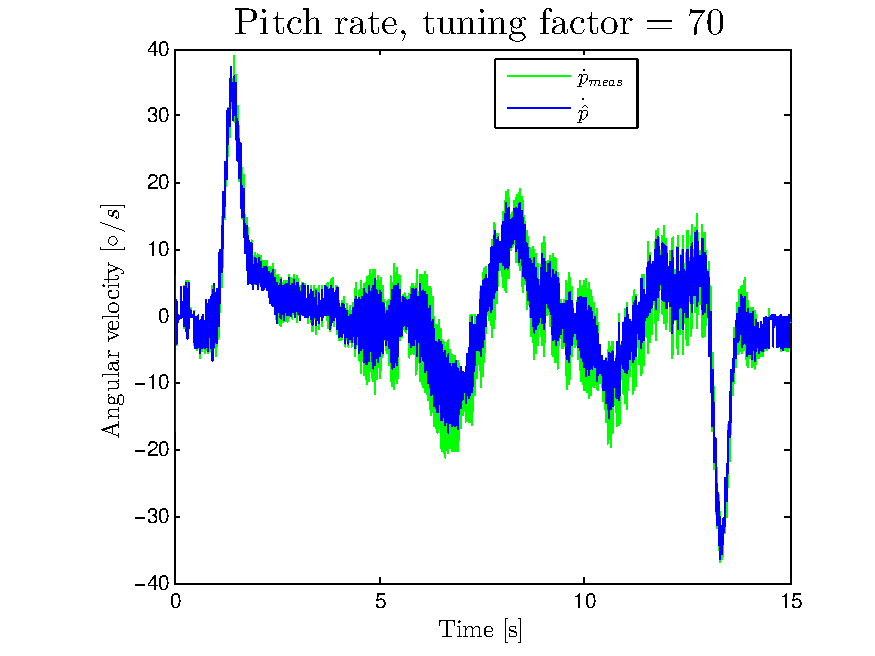
\includegraphics[width=1\textwidth,trim={0cm 0cm 0cm 0cm},clip]{figures/P4p2_pitch_rate_tuning_factor_70.pdf}
    	\caption{Pitch rate with moderate estimator}
        \label{fig:P4p2_pitch_rate_70}
    \end{minipage}    
    \begin{minipage}{0.5\textwidth}
    	\centering
		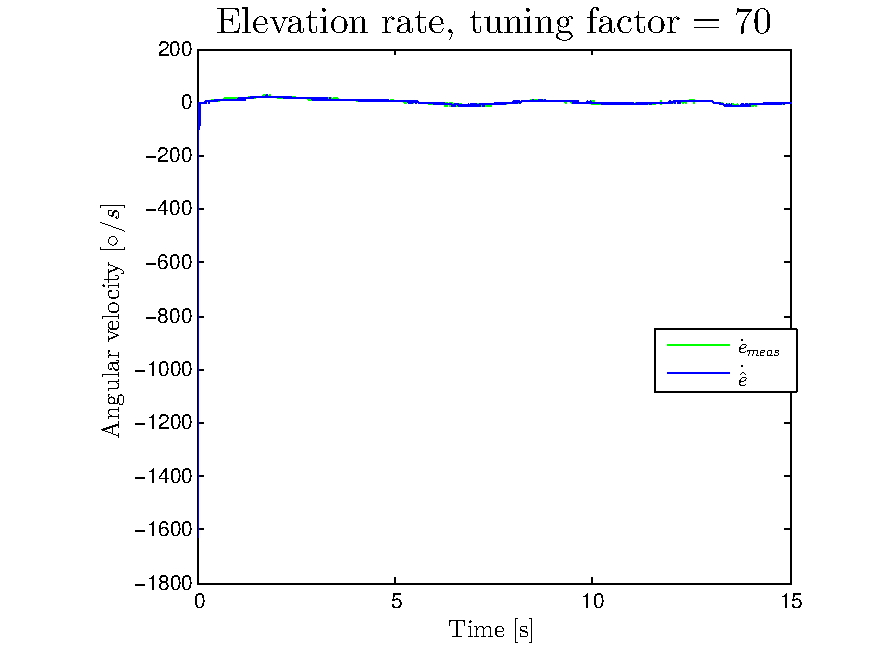
\includegraphics[width=1\textwidth,trim={0cm 0cm 0cm 0cm},clip]{figures/P4p2_elevation_rate_tuning_factor_70.pdf}
    	\caption{Elevation rate with moderate estimator}
    \label{fig:P4p2_elevation_rate_70}
    \end{minipage}    
\end{figure}
\begin{figure}[htb]
    \begin{minipage}{0.5\textwidth}
    	\centering
		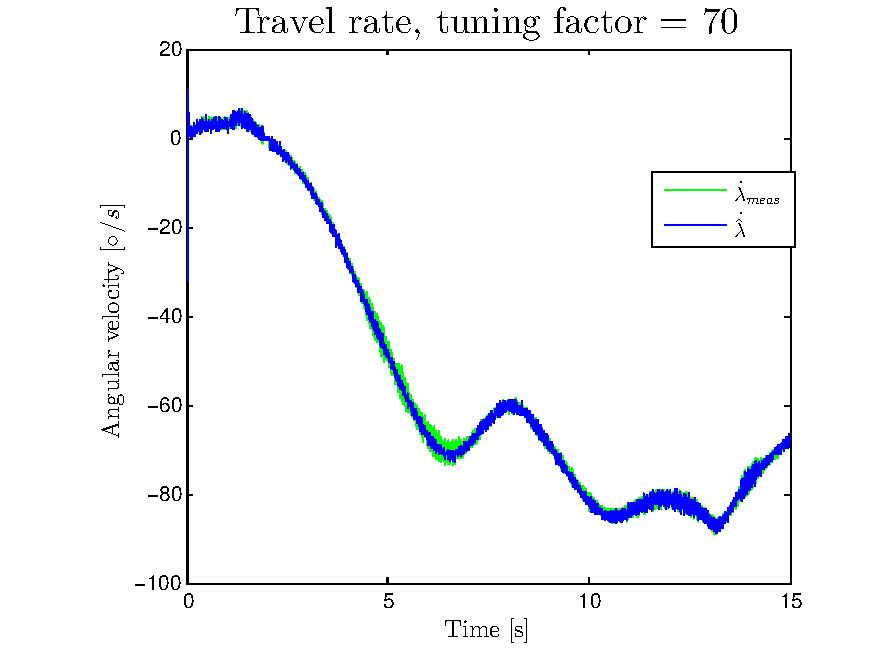
\includegraphics[width=1\textwidth,trim={0cm 0cm 0cm 0cm},clip]{figures/P4p2_travel_rate_tuning_factor_70.pdf}
    	\caption{Travel rate with moderate observer}
        \label{fig:P4p2_travel_rate_70}
    \end{minipage}    
    \begin{minipage}{0.5\textwidth}
    	\centering
		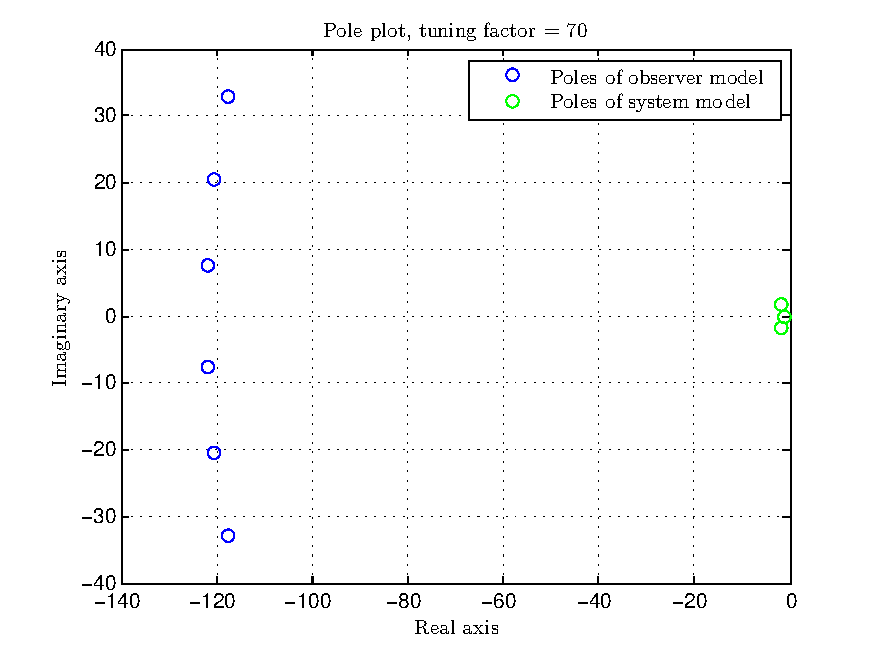
\includegraphics[width=1\textwidth,trim={0cm 0cm 0cm 0cm},clip]{figures/P4p2_pole_plot_tuning_factor_70.pdf}
    	\caption{Pole plot with moderate observer}
        \label{fig:P4p2_pole_plot_70}
    \end{minipage}    
\end{figure}
\subsubsection{Problem 3}
\textbf{Observability Analysis}\\
The matrices 
\begin{equation}
    \mathbf{C}_{e\lambda} = \begin{bmatrix}
    0 & 0 & 1 & 0 & 0 & 0 \\
    0 & 0 & 0 & 0 & 1 & 0
    \end{bmatrix}
    \quad \text{and} \quad
    \mathbf{C}_{pe} = \begin{bmatrix}
    1 & 0 & 0 & 0 & 0 & 0 \\
    0 & 0 & 1 & 0 & 0 & 0
    \end{bmatrix}
\end{equation}
correspond to the measurement vectors
\begin{equation}
    \mathbf{y}_{e\lambda} = \begin{bmatrix}
        \tilde e \\
        \tilde \lambda
    \end{bmatrix}
    \quad \text{and} \quad
    \mathbf{y}_{pe} = \begin{bmatrix}
        \tilde p \\
        \tilde e 
    \end{bmatrix}
\end{equation}
respectively.\\
Since the observability matrix,
\begin{equation}
    \setstackgap{L}{1.1\baselineskip}
    \fixTABwidth{T}
    \mathbf{\mathcal{O}}_{e\lambda} = 
        \begin{bmatrix}
        \mathbf{C}_{e\lambda}               \\
        \mathbf{C}_{e\lambda}\mathbf{A}     \\
        \mathbf{C}_{e\lambda}\mathbf{A^2}   \\
        \mathbf{C}_{e\lambda}\mathbf{A^3}   \\
        \mathbf{C}_{e\lambda}\mathbf{A^4}   \\
    \end{bmatrix}
    = \bracketMatrixstack{
    0       & 0       & 1 & 0 & 0 & 0 \\
    0       & 0       & 0 & 0 & 1 & 0 \\
    0       & 0       & 0 & 1 & 0 & 0 \\
    0       & 0       & 0 & 0 & 0 & 1 \\
    0       & 0       & 0 & 0 & 0 & 0 \\
    -0.612  & 0       & 0 & 0 & 0 & 0 \\
    0       & 0       & 0 & 0 & 0 & 0 \\
    0       & -0.612  & 0 & 0 & 0 & 0 \\
    0       & 0       & 0 & 0 & 0 & 0 \\
    0       & 0       & 0 & 0 & 0 & 0 \\
    0       & 0       & 0 & 0 & 0 & 0 \\
    0       & 0       & 0 & 0 & 0 & 0 }
\end{equation}
has full column rank, the system is observable when measuring only $\tilde e$ and $\tilde \lambda$. On the other hand, when measuring only $\tilde p$ and $\tilde e$, the system is \textit{not} observable, as

\begin{equation}
    \mathbf{\mathcal{O}}_{pe} = 
        \begin{bmatrix}
        \mathbf{C}_{pe}               \\
        \mathbf{C}_{pe}\mathbf{A}     \\
        \mathbf{C}_{pe}\mathbf{A^2}   \\
        \mathbf{C}_{pe}\mathbf{A^3}   \\
        \mathbf{C}_{pe}\mathbf{A^4}   \\
    \end{bmatrix}
    = \begin{bmatrix}
    1 & 0 & 0 & 0 & 0 & 0 \\
    0 & 0 & 1 & 0 & 0 & 0 \\
    0 & 1 & 0 & 0 & 0 & 0 \\
    0 & 0 & 0 & 1 & 0 & 0 \\
    0 & 0 & 0 & 0 & 0 & 0 \\
    0 & 0 & 0 & 0 & 0 & 0 \\
    0 & 0 & 0 & 0 & 0 & 0 \\
    0 & 0 & 0 & 0 & 0 & 0 \\
    0 & 0 & 0 & 0 & 0 & 0 \\
    0 & 0 & 0 & 0 & 0 & 0 \\
    0 & 0 & 0 & 0 & 0 & 0 \\
    0 & 0 & 0 & 0 & 0 & 0 \\
    \end{bmatrix}
\end{equation}
does \textit{not} have full column rank.\\
This also makes intuitive sense, as we cannot expect to observe the travel, $\lambda$, from only knowing elevation $e$ and the pitch $p$. But if we do know the travel, the pitch can be obtained by taking the derivative.\\ 
\\
\textbf{The Baddest Observer in the West}\\
Tuning the observer based solely on the outputs $e$ and $\lambda$ proved to be much harder than when the pitch, $p$ was also part of the measurements. The erroneous estimation is most clear in the pitch rate estimation as shown in figure (WE DONT HAVE A GOOD FIGURE WAT DO). This is partly because the pitch has the non-linear correlation with elevation and travel given in equations \eqref{eq:P1_elevation_non-linear} and \eqref{eq:P1_travel_non-linear}, but the observer is based on the linearised equations given in \eqref{eq:P1_linearised_equations_of_motion}. As a result, the estimation error becomes more prevalent the further away from the linearisation point the state sways. This error gets amplified further when taking the derivative, since a high frequency noise signal such as $\sin(\omega t)$, where $\omega$ is large, has the high amplitude derivative $\omega \cos(\omega t)$. 
    

% Conclusion

\section{Conclusion}\label{sec:conclusion}
This does not have to be long, but try to write a few reasonable closing remarks.


% Appendix

\addcontentsline{toc}{section}{Appendix} % Remove this if you don't want the appendix included in the table of contents.
\appendix

\section{MATLAB Code}\label{sec:matlab}
This section should contain your MATLAB code. DO NOT attach files posted online (that you didn't write). Note that the method used to input code below does not look as pretty when the lines are too long.

\subsection{plot\_constraint.m}\label{sec:plot_constraint_m}
\lstinputlisting{code/plot_constraint.m}\section{Simulink Diagrams}\label{sec:simulink}
This section should contain your Simulink diagrams. Just like the plots, these should be in vector format, like in \Cref{fig:simulink}. Make them tidy enough to understand.

\subsection{Simulink Diagrams for Part II}
\begin{figure}[!!ht!!!!!!!!tb!!]
    	\centering
		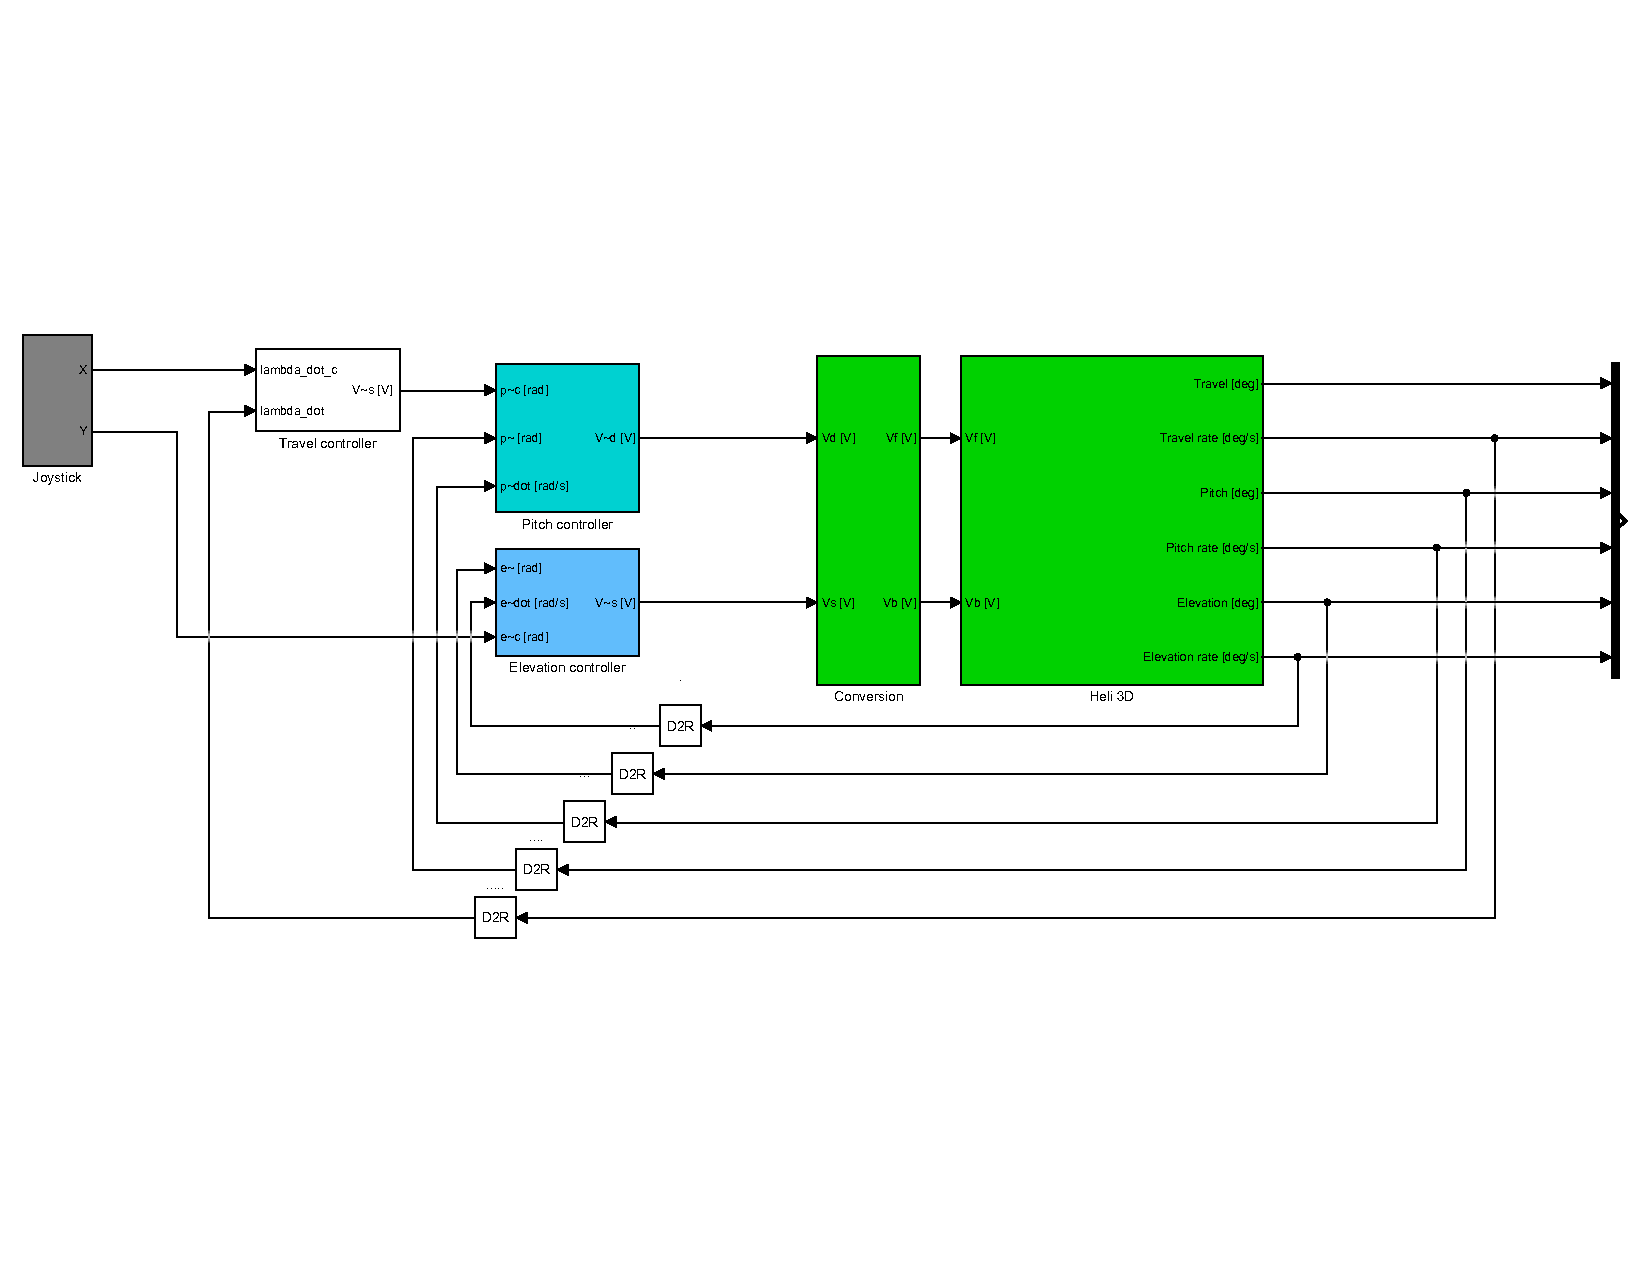
\includegraphics[width=1.1\textwidth,trim={0cm 3cm 0cm 5cm},clip]{figures/simulink/P2p2.pdf}
    	\caption{Top view of model from Part 2 problem 2}
\label{fig:P2p2_simulink}
\end{figure}
\FloatBarrier

\section{Parameters and values}\label{sec:parameters}


\begin{table}[tbp]
	\centering
	\caption{Parameters and values.}
	\begin{tabular}{llll}
		\toprule
		Symbol & Parameter & Value & Unit \\
		\midrule
		$l_h$ & Distance from elevation axis to helicopter body & $0.63$  & \meter                      \\
		$l_p$ & Distance from pitch axis to motor               & $0.18$  & \meter                      \\
		$K_f$ & Force constant motor                            & $0.25$  & \newton\per\volt            \\
		$J_e$ & Moment of inertia for elevation                 & $0.83$  & \kilogram\usk\meter\squared \\
$J_{\lambda}$ & Moment of inertia for travel                    & $0.83$  & \kilogram\usk\meter\squared \\
		$J_p$ & Moment of inertia for pitch                     & $0.034$ & \kilogram\usk\meter\squared \\
		$m_p$ & Mass of helicopter                              & $1.05$  & \kilogram                   \\
		$m_c$ & Weight of counterweight                         & $1.87$  & \kilogram                   \\
		\bottomrule
	\end{tabular}
\label{tab:parameters}
\end{table}

% \input simply inserts the contents of the file, while \include forces a \newpage.
% See \input vs. \include: http://tex.stackexchange.com/questions/246/when-should-i-use-input-vs-include

% References
\newpage
\addcontentsline{toc}{section}{References}
\printbibliography{}
\label{sec:bibliography}

\end{document}


\section{HOW-TO Rapport}\label{sec:howto} % TODO: Remove
Your introduction should contain an overview of the work you were assigned, as well as a few sentences putting the work into a larger perspective. You should also give a quick description of how the report is organized (as is done below).

You should of course put most of the work into doing good work in the lab and then presenting it in the report. When presenting your work in the report, both content and presentation/layout matters. Since your only way of communicating your good effort in the lab is through writing about it here, the way you write about it is essential. This means that even if you have the very best controller but describe it poorly, you will probably not be rewarded for the good results. A plot showing perfect control is worth very little if it is not accompanied by a clear description of what it represents.

Layout is naturally less important than content, but it still matters. You can think of report writing like selling an apartment; when you present your apartment for potential buyers you will of course clean the apartment and make it good looking. How clean the apartment is does of course not determine its value, but it is still important since it influences the subjective value your buyers will put on the apartment. 
